\section{Constructions at \Fii{}}\label{sec:f2}

The first classes \Fii{} has to reach are the Weil classes of a very general abelian $2n$-fold of Weil type with $n\ge3$, and the exceptional classes of a Mumford fourfold. We build an object at each.

\subsection{The polarised semiregularity criterion}\label{ssec:criterion}

Let $A$ be a very general member of the polarised family $\cD_{n,n}$ of abelian $2n$-folds of Weil type for an imaginary quadratic field $K$, with polarisation class $\theta$ and Weil plane $W(A)$. Then $\Hdg^{*}(A)=\QQ[\theta]\oplus W(A)$ and $W(A)\cdot\theta=0$ \cite[Thm.~4.14]{BMB26}. A class $\gamma\in H^{\mathrm{ev}}(A)$ has the polarised shape if
\[
\gamma=N\omega+\sum_{k=0}^{2n}c_{k}\theta^{k},\qquad N\ne0,\ 0\ne\omega\in W(A),\ c_{k}\in\QQ .
\]
Its Hankel rank $\rho\in\{0,1,2,3\}$ is the rank of the Hankel matrix of the sequence $(k!\,c_{k})_{k}$ capped at three; it is the number of distinct exponentials $e^{a\theta}$ needed to write the polynomial part when that number is at most two, and $3$ otherwise.\footnote{The Hankel matrix of a sequence $(a_{k})_{k\ge0}$ has entries $a_{i+j}$. If $a_{k}$ is a sum $\sum_{j}\lambda_{j}b_{j}^{k}$ of $m$ terms with distinct $b_{j}$ and nonzero $\lambda_{j}$, the matrix factors as $V^{\mathsf{T}}\operatorname{diag}(\lambda_{j})V$ with $V$ the Vandermonde matrix of the $b_{j}$, so its rank is $m$; conversely a sequence whose Hankel matrix has finite rank $m$ satisfies a linear recurrence of order $m$ and is a sum of $m$ exponentials with polynomial coefficients. For the polynomial part $\sum_{k}c_{k}\theta^{k}$ of a Chern character, writing it as $\sum_{j}\lambda_{j}e^{b_{j}\theta}$ means $k!\,c_{k}=\sum_{j}\lambda_{j}b_{j}^{k}$, so the number of exponentials needed is the Hankel rank of $(k!\,c_{k})$, provided the degree $2n$ allows the recurrence to be read off, which it does for $m\le2$; the cap at three records that the criterion of Theorem~\ref{thm:criterion} does not distinguish further.}

\begin{theorem}[The polarised criterion \protect{\cite{BMB26}}]\label{thm:criterion}
Let $\mathcal{E}$ be a perfect complex on $A$ with $\ch(\mathcal{E})=\gamma$ of polarised shape and Hankel rank $\rho$. Then
\[
\dim\Ext^{2}(\mathcal{E},\mathcal{E})\ \ge\ r(\gamma):=(4+\rho)\,n^{2}-2n,
\]
and if equality holds the semiregularity map\footnote{For a perfect complex $\mathcal{E}$ on a smooth projective variety the semiregularity map of Buchweitz and Flenner \cite{BF03} is the linear map $\sigma_{\mathcal{E}}\colon\Ext^{2}(\mathcal{E},\mathcal{E})\to\prod_{q}H^{q+1}(X,\Omega^{q-1}_{X})$ sending $\xi$ to the trace of $\xi\circ\exp\bigl(-\mathrm{At}(\mathcal{E})\bigr)$, where $\mathrm{At}(\mathcal{E})\in\Ext^{1}(\mathcal{E},\mathcal{E}\otimes\Omega^{1}_{X})$ is the Atiyah class; it generalises Bloch's map for a subvariety \cite{Blo72}, which is the case of the structure sheaf of the subvariety. Its value is that the obstruction to deforming $\mathcal{E}$ along a first-order deformation of $X$ lies in $\Ext^{2}(\mathcal{E},\mathcal{E})$ and is sent by $\sigma_{\mathcal{E}}$ to the obstruction to keeping $\ch(\mathcal{E})$ of Hodge type; so when $\sigma_{\mathcal{E}}$ is injective, $\mathcal{E}$ deforms wherever its Chern character stays a Hodge class, and the Chern character of the deformed complex is algebraic there. The dimension count of the theorem is the arithmetic of this statement: the rank of $\sigma_{\mathcal{E}}$ is at least the rank of the contraction into $\ch(\mathcal{E})$, so $\dim\Ext^{2}$ is at least $r(\gamma)$, and equality forces injectivity.} of $\mathcal{E}$ is injective, $\mathcal{E}$ deforms with $A$ along the whole of $\cD_{n,n}$, and the Weil classes are algebraic on every member of the family with full Hodge group. If some $c_{k}\ne0$ with $1\le k\le 2n-1$, the first-order Hodge locus of $\gamma$ in $H^{1}(A,T_{A})$ is the tangent space of $\cD_{n,n}$, of dimension $n^{2}$. A perfect complex whose Chern character is exactly a multiple of a Weil class does not exist on a very general member, so the polynomial part is forced.
\end{theorem}

The number $r(\gamma)$ is the rank of the contraction $HT^{2}(A)\to H^{*}(A)$, $\xi\mapsto\xi\lrcorner\gamma$, on the Hochschild cohomology $HT^{2}=\bigoplus_{p+q=2}H^{q}(A,\bigwedge^{p}T_{A})$, of dimension $\binom{4n}{2}$; its kernel is the annihilator $\mathrm{Ann}(\gamma)$, which meets $H^{1}(A,T_{A})$ in the first-order Hodge locus. The semiregularity map $\sigma_{\mathcal{E}}$ of a perfect complex composes with the characteristic map $\mathrm{ev}_{\mathcal{E}}:HT^{2}\to\Ext^{2}(\mathcal{E},\mathcal{E})$, $\xi\mapsto\xi\lrcorner\mathrm{At}(\mathcal{E})$, to the contraction into $\ch(\mathcal{E})$; this is how the lower bound arises, and it is the form in which the criterion is used below. Figure~\ref{fig:hankel} shows $r(\gamma)$; the two values that matter below are $r=57$ at $n=3$, $\rho=3$ and $r=104$ at $n=4$, $\rho=3$. On the product $E_{0}^{6}$ of six copies of the elliptic curve $\CC/\ZZ[i]$ every twisted complex of line bundles has $\dim\Ext^{2}\ge69>57$ \cite[Thm.~18.35]{BMB26}; the criterion is not met there by any such object.

\begin{figure*}[t]
\centering
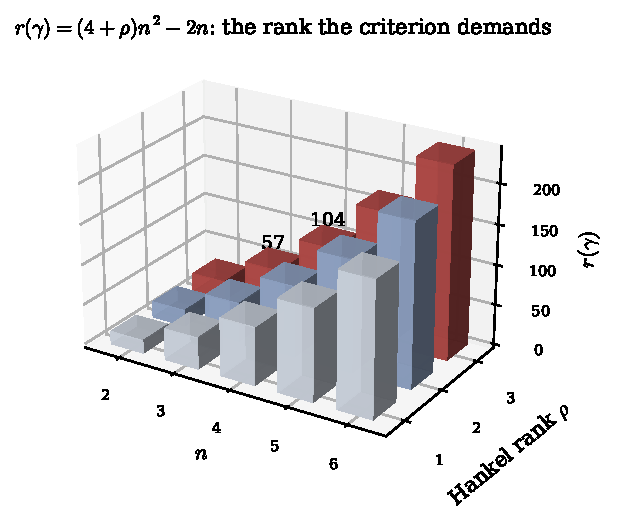
\includegraphics[width=0.78\textwidth]{figures/fig_hankel}
\caption{The lower bound $r(\gamma)=(4+\rho)n^{2}-2n$ of Theorem~\ref{thm:criterion} for $2\le n\le6$ and Hankel rank $\rho=1,2,3$. The two labelled bars are the product cases of Theorem~\ref{thm:product}.}
\label{fig:hankel}
\end{figure*}

\subsection{The Weil plane of a product}

\begin{lemma}\label{lem:weilproduct}
Let $A$, $A'$ be of Weil type for the same field $K$, of dimensions $2m$, $2m'$, with the diagonal $K$-action on $A\times A'$. Then $W(A\times A')$ is a two-dimensional rational subspace of the four-dimensional space $W(A)\otimes W(A')\subseteq H^{2n}(A\times A')$, $n=m+m'$, and every rational $w\in W(A\times A')$ is $\sum_{i,j}a_{ij}\,\omega_{i}\otimes\omega'_{j}$ with $a_{ij}\in\QQ$ for rational bases $(\omega_{i})$, $(\omega'_{j})$ of $W(A)$, $W(A')$.
\end{lemma}

\begin{proof}
Over $\CC$, $H^{1}(A\times A')=V\oplus V'$ splits into eigenspaces $V_{\pm}\oplus V'_{\pm}$ of $K$, and $\bigwedge^{2n}_{K}$ of the sum is spanned by $\det V_{+}\otimes\det V'_{+}$ and $\det V_{-}\otimes\det V'_{-}$; these lie in the span of the four products $\omega_{\pm}\otimes\omega'_{\pm}$ of the eigenvectors of $W(A)\otimes\CC$ and $W(A')\otimes\CC$. Both $W(A\times A')$ and $W(A)\otimes W(A')$ are defined over $\QQ$, so the inclusion holds over $\QQ$. The explicit formula is \cite[Eq.~(36)]{BMB26}: $\omega_{1}(A\times A')=\omega_{1}\otimes\omega'_{1}-d\,\omega_{2}\otimes\omega'_{2}$ for $K=\QQ(\sqrt{-d})$.
\end{proof}

\subsection{An object with the polarised Chern character}

\begin{theorem}[The product object]\label{thm:product}
Let $A$, $A'$ be very general in their polarised Weil families, with ample classes $\theta_{A}$, $\theta_{A'}$, $\theta=\theta_{A}+\theta_{A'}$, and suppose that $W(A)$ and $W(A')$ are algebraic. Then there is a perfect complex $\mathcal{E}$ on $A\times A'$, a finite direct sum with shifts of exterior products
\[
F_{i}\boxtimes G'_{j},\quad F_{i}\boxtimes L'^{\,k},\quad L^{l}\boxtimes G'_{j},\quad L^{l}\boxtimes L'^{\,k},
\]
with $F_{i}$, $G'_{j}$ coherent sheaves on $A$, $A'$ and $L$, $L'$ the ample bundles, such that
\[
\ch(\mathcal{E})=N\,w+\sum_{k=0}^{2n}c_{k}\theta^{k},\qquad N\ne0,\ 0\ne w\in W(A\times A'),
\]
has the polarised shape with Hankel rank $\rho=3$, so that $r(\ch\mathcal{E})=7n^{2}-2n$, and the first-order Hodge locus of $\ch(\mathcal{E})$ in $H^{1}(A\times A',T)$ is the tangent space of $\cD_{n,n}$.
\end{theorem}

The hypotheses hold in the two open cases nearest to the known ones: $A$, $A'$ very general Weil fourfolds of trivial discriminant, where Markman proves the Weil classes algebraic \cite{Mar25a,Mar25b}, so that $A\times A'$ is an eightfold with $n=4$; and $A$ such a fourfold and $A'=B$ a Weil surface of any discriminant $d$, whose Weil plane is of type $(1,1)$ and algebraic by Lefschetz, so that $A\times B$ is a sixfold of discriminant $d$ with $n=3$.

\begin{proof}
Since $\Hdg^{*}(A)=\QQ[\theta_{A}]\oplus W(A)$, algebraic classes on $A$ are rational combinations of Chern characters of coherent sheaves, and the Chern character of a coherent sheaf is a Hodge class, the algebraicity of $W(A)$ gives coherent sheaves $F_{1}$, $F_{2}$ with $\ch(F_{i})=N_{i}\omega_{i}+p_{i}(\theta_{A})$, $N_{i}\ne0$, for a basis $(\omega_{1},\omega_{2})$ of $W(A)$; likewise $G'_{1}$, $G'_{2}$ on $A'$ with $\ch(G'_{j})=N'_{j}\omega'_{j}+p'_{j}(\theta_{A'})$. Fix $0\ne w\in W(A\times A')$ rational, $w=\sum a_{ij}\omega_{i}\otimes\omega'_{j}$ by Lemma~\ref{lem:weilproduct}, and a common denominator $M$ of the numbers $Ma_{ij}/(N_{i}N'_{j})$, so that these are integers. Negative multiplicities are realised by the shift $[1]$, which changes the sign of $\ch$.

Step 1. $\mathcal{E}_{0}=\bigoplus_{i,j}(F_{i}\boxtimes G'_{j})^{\oplus Ma_{ij}/(N_{i}N'_{j})}$ has, by multiplicativity,
\begin{widetext}
\begin{equation}\label{eq:chE0}
\ch(\mathcal{E}_{0})=Mw+\sum_{i}\omega_{i}\otimes q'_{i}(\theta_{A'})+\sum_{j}q_{j}(\theta_{A})\otimes\omega'_{j}+s,
\end{equation}
\end{widetext}
with $q'_{i}$, $q_{j}$ polynomials and $s\in\QQ[\theta_{A}]\otimes\QQ[\theta_{A'}]$.

Step 2. The classes $e^{k\theta_{A'}}=\ch(L'^{\,k})$, $k=0,\dots,2m'$, form a basis of $\QQ[\theta_{A'}]/(\theta_{A'}^{2m'+1})$: the matrix $(k^{j}/j!)_{j,k}$ has determinant $\prod_{j}(1/j!)$ times the Vandermonde determinant of $0,1,\dots,2m'$, which is nonzero. Write $q'_{i}=\sum_{k}b_{ik}e^{k\theta_{A'}}$ and add $(F_{i}\boxtimes L'^{\,k})^{\oplus-Mb_{ik}/N_{i}}$, after enlarging $M$ to clear denominators; this removes $\omega_{i}\otimes q'_{i}$ and adds only terms $p_{i}(\theta_{A})\otimes e^{k\theta_{A'}}$, which lie in $\QQ[\theta_{A}]\otimes\QQ[\theta_{A'}]$. Symmetrically remove $q_{j}\otimes\omega'_{j}$ with summands $L^{l}\boxtimes G'_{j}$.

\begin{figure*}[t]
\centering
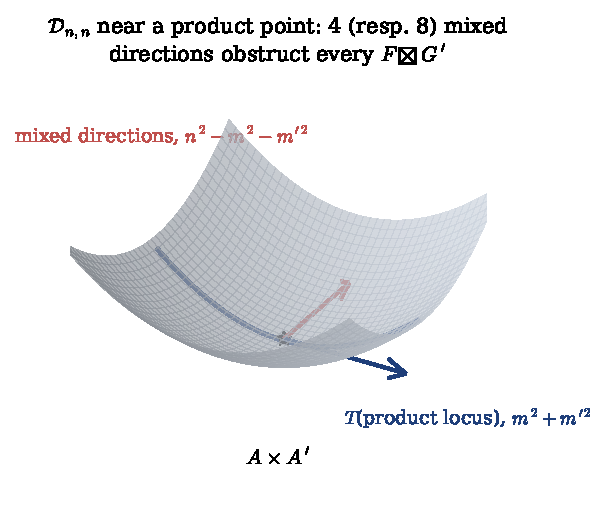
\includegraphics[width=0.78\textwidth]{figures/fig_product}
\caption{The domain $\cD_{n,n}$ near a product point $A\times A'$. The curve is the product locus, whose tangent space has dimension $m^{2}+m'^{2}$; the $2mm'$ mixed directions obstruct every exterior product $F\boxtimes G'$, and only the combined object of Theorem~\ref{thm:product} has the full tangent space as first-order Hodge locus.}
\label{fig:product}
\end{figure*}

Step 3. The classes $e^{l\theta_{A}+k\theta_{A'}}=\ch(L^{l}\boxtimes L'^{\,k})$ form a basis of $\QQ[\theta_{A}]/(\theta_{A}^{2m+1})\otimes\QQ[\theta_{A'}]/(\theta_{A'}^{2m'+1})$ by the same determinant, so the remaining part in $\QQ[\theta_{A}]\otimes\QQ[\theta_{A'}]$ is cancelled by line bundles with integer multiplicities and shifts. Finally add $(L\boxtimes L')^{\otimes k}$, $k=0,1,2$, with generic nonzero multiplicities $\mu_{k}$. The result is
\[
\ch(\mathcal{E})=Mw+\sum_{k=0}^{2}\mu_{k}e^{k\theta},
\]
a polarised shape whose polynomial part is a sum of three distinct exponentials with nonzero coefficients. Three exponentials are not one of the shapes of Hankel rank at most two, so $\rho=3$; and some $c_{k}$ with $1\le k\le2n-1$ is nonzero, so the first-order Hodge locus is the tangent space of $\cD_{n,n}$ by Theorem~\ref{thm:criterion}.
\end{proof}

The construction was carried out in the exterior-algebra model of $H^{*}(A\times A')$ for $(m,m')=(2,1)$ and $(2,2)$: the cross terms of $\ch(\mathcal{E}_{0})$ vanish, nothing is left outside $W(A\times A')\oplus\QQ[\theta]$ after Steps 2 and 3, the Hankel rank is $3$, and the first-order Hodge locus has dimension $9$, resp.\ $16$, equal to $n^{2}$ (Appendix~\ref{app:checks}).

\subsection{What a direct sum cannot do}

The tangent space of $\cD_{n,n}$ at a product point contains the tangent space of the product locus $\cD_{m,m}\times\cD_{m',m'}$, of dimension $m^{2}+m'^{2}$, and $n^{2}-m^{2}-m'^{2}=2mm'$ mixed directions. In the same model, each exterior product $F\boxtimes G'$ of sheaves of polarised shape has first-order Hodge locus inside $T\cD_{n,n}$ equal to the tangent space of the product locus: all $2mm'$ mixed directions obstruct it, four for $A\times B$ and eight for $A\times A'$ (Fig.~\ref{fig:product}). The object $\mathcal{E}$ of Theorem~\ref{thm:product} has the whole tangent space as its first-order locus because its Chern character is a single polarised class and not a product. Semiregularity is a different matter.

\begin{proposition}[Direct sums are never semiregular]\label{prop:directsum}
\leavevmode
\begin{enumerate}[label=\textup{(\roman*)},leftmargin=2.4em,itemsep=2pt]
\item Let $\mathcal{E}=\bigoplus_{k}\mathcal{E}_{k}$ be a direct sum of at least two nonzero complexes. Then the semiregularity map $\sigma_{\mathcal{E}}$ vanishes on $\bigoplus_{k\ne l}\Ext^{2}(\mathcal{E}_{k},\mathcal{E}_{l})$. So $\sigma_{\mathcal{E}}$ is injective only if $\Ext^{2}(\mathcal{E}_{k},\mathcal{E}_{l})=0$ for all $k\ne l$.
\item For every direct-sum realisation $\mathcal{E}$ of Theorem~\ref{thm:product}, $\sigma_{\mathcal{E}}$ is not injective and $\dim\Ext^{2}(\mathcal{E},\mathcal{E})>r(\ch\mathcal{E})$.
\end{enumerate}
\end{proposition}

\begin{proof}
(i) The semiregularity map of Buchweitz and Flenner is built from the traces $\xi\mapsto\mathrm{tr}\bigl(\xi\circ\mathrm{At}(\mathcal{E})^{p}\bigr)$ of compositions with powers of the Atiyah class \cite[Sect.~4]{BF03}. The Atiyah class of a direct sum is block diagonal, so for $\xi$ in an off-diagonal block $\Ext^{2}(\mathcal{E}_{k},\mathcal{E}_{l})$ the composition $\xi\circ\mathrm{At}(\mathcal{E})^{p}$ is off-diagonal, and the trace of an off-diagonal block is zero.

(ii) The summands of $\mathcal{E}$ include $F_{1}\boxtimes L'^{\,k}$ and $F_{1}\boxtimes L'^{\,l}$ for two exponents $k<l$, because Step 2 of the proof uses every power $L'^{\,k}$ with $0\le k\le2m'$ (the exponentials form a basis and $q'_{1}$ is a nonzero polynomial of positive degree for a sheaf of polarised shape, which has $p_{1}$ of positive degree by Theorem~\ref{thm:criterion}). By the K\"unneth formula
\begin{widetext}
\begin{equation}\label{eq:kunneth}
\Ext^{2}(F_{1}\boxtimes L'^{\,k},F_{1}\boxtimes L'^{\,l})\supseteq\Ext^{2}(F_{1},F_{1})\otimes H^{0}(A',L'^{\,l-k}),
\end{equation}
\end{widetext}
and $\dim\Ext^{2}(F_{1},F_{1})\ge r(\ch F_{1})\ge12$ by Theorem~\ref{thm:criterion} on the fourfold $A$ ($n=2$, $\rho\ge0$), while $H^{0}$ of an ample bundle is nonzero. So an off-diagonal block is nonzero, $\sigma_{\mathcal{E}}$ has a kernel by (i), and $\dim\Ext^{2}(\mathcal{E},\mathcal{E})>r$ because equality would force injectivity.
\end{proof}

\begin{proposition}[Convolutions]\label{prop:convolution}
Let $\mathcal{E}_{\delta}$ be a one-sided twisted complex on pieces $P_{1},\dots,P_{N}$ with shifts $s_{a}$, ordered so that the differential $\delta=(\delta_{ab})_{a<b}$, $\delta_{ab}\in\Ext^{1+s_{a}-s_{b}}(P_{a},P_{b})$, is strictly upper triangular; let $\gamma=\ch(\mathcal{E}_{\delta})=\sum_{a}(-1)^{s_{a}}\ch(P_{a})$.
\begin{enumerate}[label=\textup{(\roman*)},leftmargin=2.4em,itemsep=2pt]
\item The semiregularity map $\sigma_{\mathcal{E}_{\delta}}$ vanishes on every class of $\Ext^{2}(\mathcal{E}_{\delta},\mathcal{E}_{\delta})$ represented by a strictly upper triangular cocycle. So the criterion holds for $\mathcal{E}_{\delta}$ only if every strictly upper triangular cocycle of degree two is a coboundary.
\item Suppose no term of the twisted differential carries a class of degree one into a diagonal block $\Ext^{*}(P_{c},P_{c})$. Let $v\in T\cD_{n,n}$ have a nonzero mixed component. If some piece $P=X\boxtimes Y$ has $\operatorname{rk}Y\,c_{1}(X)/\theta_{A}\ne\operatorname{rk}X\,c_{1}(Y)/\theta_{A'}$, then $\mathrm{ev}_{\mathcal{E}_{\delta}}(v)\ne0$ and $\sigma_{\mathcal{E}_{\delta}}(\mathrm{ev}_{\mathcal{E}_{\delta}}(v))=0$: the criterion fails.
\item Suppose the pieces split into two nonempty groups with $\Ext^{*}(P_{a},P_{b})=0$ in both directions for $a$, $b$ in different groups. Then $\mathcal{E}_{\delta}=\mathcal{E}'\oplus\mathcal{E}''$ is the direct sum of the convolutions of the groups, and the criterion holds for $\mathcal{E}_{\delta}$ only if every $v\in T\cD_{n,n}$ annihilates $\ch(\mathcal{E}')$ and $\ch(\mathcal{E}'')$ separately.
\end{enumerate}
\end{proposition}

\begin{proof}
(i) The components of $\sigma_{\mathcal{E}_{\delta}}(\xi)$ are the traces $\mathrm{tr}(\xi\circ\mathrm{At}(\mathcal{E}_{\delta})^{p})/p!$ \cite[Sect.~4]{BF03}. In the harmonic model of a twisted complex the Atiyah class is represented by $[\nabla,\bar\partial+\delta]$ with $\nabla$ the direct sum of the Chern connections of the pieces; it is block upper triangular with diagonal blocks $\mathrm{At}(P_{a})$ and off-diagonal blocks $\nabla\delta_{ab}$. The homotopy transfer $\xi\mapsto\sum_{k}(-h[\delta,\,\cdot\,])^{k}\xi$ that produces the chain-level representative of $\xi$ raises or preserves the block position $b-a$, so a strictly upper triangular cocycle has a strictly upper triangular representative. The product of an upper triangular block matrix with a strictly upper triangular one is strictly upper triangular, and its trace, the sum of the traces of its diagonal blocks, is zero. The trace is a chain map for $\bar\partial+[\delta,\,\cdot\,]$ by cyclicity, so the vanishing holds in cohomology. Since $\sigma_{\mathcal{E}_{\delta}}\circ\mathrm{ev}_{\mathcal{E}_{\delta}}$ is contraction into $\gamma$, of rank $r(\gamma)$, the kernel of $\sigma_{\mathcal{E}_{\delta}}$ contains the image of the strictly upper triangular classes and $\dim\Ext^{2}\ge r(\gamma)+\dim(\text{that image})$.

(ii) The Atiyah class of $X\boxtimes Y$ is $\mathrm{At}(X)\otimes1+1\otimes\mathrm{At}(Y)$, so the diagonal component of $\mathrm{ev}_{\mathcal{E}_{\delta}}(v)$ at $P$ is $v\lrcorner\mathrm{At}(P)$, with trace $v\lrcorner\ch_{1}(P)$. Write $v=v_{A}+v_{A'}+z\otimes d'+z'\otimes d$ with $v_{A}\in T\cD_{m,m}$, $v_{A'}\in T\cD_{m',m'}$, $z\in H^{0,1}(A)$, $d'\in H^{0}(T_{A'})$, $z'\in H^{0,1}(A')$, $d\in H^{0}(T_{A})$. Since $v$ kills $\theta=\theta_{A}+\theta_{A'}$ and $v_{A}\lrcorner\theta_{A}=v_{A'}\lrcorner\theta_{A'}=0$, we have $v\lrcorner\theta_{A'}=-v\lrcorner\theta_{A}=-z'\wedge(d\lrcorner\theta_{A})$, nonzero when $d\ne0$ because $\theta_{A}$ is nondegenerate and $z'\wedge$ is injective on $H^{0,1}(A)$; the case $d=0$, $d'\ne0$ is symmetric. On a very general member $c_{1}(X)$ and $c_{1}(Y)$ are multiples of the polarisations, so $v\lrcorner\ch_{1}(P)=\bigl(\operatorname{rk}Y\,c_{1}(X)/\theta_{A}-\operatorname{rk}X\,c_{1}(Y)/\theta_{A'}\bigr)\,v\lrcorner\theta_{A}\ne0$ under the hypothesis on $P$. Under the assumption on the differential, the diagonal components of a class in $\Ext^{2}(\mathcal{E}_{\delta},\mathcal{E}_{\delta})$ are well defined, so $\mathrm{ev}_{\mathcal{E}_{\delta}}(v)\ne0$, while $\sigma_{\mathcal{E}_{\delta}}(\mathrm{ev}_{\mathcal{E}_{\delta}}(v))=v\lrcorner\gamma=0$ because $v$ is tangent to the Hodge locus of $\gamma$.

(iii) With no Ext groups between the groups there are no components of $\delta$ between them, so the twisted complex is block diagonal,
\begin{widetext}
\begin{equation}\label{eq:blockdiag}
\Ext^{2}(\mathcal{E}_{\delta},\mathcal{E}_{\delta})=\Ext^{2}(\mathcal{E}',\mathcal{E}')\oplus\Ext^{2}(\mathcal{E}'',\mathcal{E}''),\qquad
\dim\Ext^{2}(\mathcal{E}_{\delta},\mathcal{E}_{\delta})\ge\dim HT^{2}-\dim\bigl(\mathrm{Ann}(\ch\mathcal{E}')\cap\mathrm{Ann}(\ch\mathcal{E}'')\bigr),
\end{equation}
\end{widetext}
with $\sigma_{\mathcal{E}_{\delta}}=\sigma_{\mathcal{E}'}\oplus\sigma_{\mathcal{E}''}$; the inequality holds because for each summand the contraction into its Chern character factors through $\mathrm{ev}$ and $\sigma$, so that $\dim\Ext^{2}(\mathcal{E}',\mathcal{E}')$ is at least the rank of $\xi\mapsto\xi\lrcorner\ch\mathcal{E}'$, and likewise for $\mathcal{E}''$. Here $r(\gamma)=\dim HT^{2}-\dim\mathrm{Ann}(\gamma)$ with $\mathrm{Ann}(\gamma)=T\cD_{n,n}$. Equality $\dim\Ext^{2}=r(\gamma)$ forces the common annihilator to be all of $T\cD_{n,n}$.
\end{proof}

For the pieces of Theorem~\ref{thm:product} the splitting in (iii) that one would like to use separates the pieces $F_{i}\boxtimes Y$ carrying a secant sheaf on $A$ from the pieces $L^{l}\boxtimes Y'$. Two statements settle what that splitting gives. The first computes the annihilator of the secant pieces by hand; the second shows that the splitting is never available.

\begin{theorem}[The annihilator of the secant pieces]\label{thm:annihilator}
Let $\mathcal{E}'$ be the sum, with the multiplicities and shifts of Theorem~\ref{thm:product}, of the pieces $F_{i}\boxtimes G'_{j}$ and $F_{i}\boxtimes L'^{\,k}$. Then
\begin{equation}\label{eq:chEprime}
\ch(\mathcal{E}')=Mw+\sum_{i}\frac{M}{N_{i}}\,p_{i}(\theta_{A})\otimes R_{i},\qquad R_{i}=\sum_{j}a_{ij}\omega'_{j},
\end{equation}
where $(a_{ij})$ is the matrix of $w$ in the bases $(\omega_{i})$, $(\omega'_{j})$ and is invertible, and the annihilator of $\ch(\mathcal{E}')$ in $T\cD_{n,n}$ is the tangent space $T\cD_{m,m}\oplus T\cD_{m',m'}$ of the product locus, of dimension $m^{2}+m'^{2}$. If $\Ext^{*}(F_{i},L^{l})=0$ for every power $L^{l}$ among the pieces, every convolution $\mathcal{E}_{\delta}$ of the pieces has $\dim\Ext^{2}(\mathcal{E}_{\delta},\mathcal{E}_{\delta})\ge r(\gamma)+2mm'$, which is $61$ at $n=3$ and $120$ at $n=4$.
\end{theorem}

\begin{proof}
Steps 1 and 2 of Theorem~\ref{thm:product} add and subtract, for each $i$, the classes
\[
\sum_{j}\frac{Ma_{ij}}{N_{i}N'_{j}}\,\ch(F_{i})\ch(G'_{j})\quad\text{and}\quad\frac{M}{N_{i}}\,\ch(F_{i})\otimes q'_{i},
\]
where $q'_{i}=\sum_{j}(a_{ij}/N'_{j})p'_{j}$; the difference is $\ch(F_{i})\otimes R_{i}$, and summing over $i$ with $\ch(F_{i})=N_{i}\omega_{i}+p_{i}(\theta_{A})$ gives \eqref{eq:chEprime}, the terms $\omega_{i}\otimes R_{i}$ adding up to $Mw$ by the definition of $a$. By Lemma~\ref{lem:weilproduct} $w=x\,\omega_{+}\otimes\omega'_{+}+\bar x\,\omega_{-}\otimes\omega'_{-}$ with $x\ne0$, a tensor of rank two, so $a$ is invertible and $R_{1}$, $R_{2}$ form a basis of the Weil plane of $A'$.

Write $V=H^{1}(A,\CC)=V_{+}\oplus V_{-}$ for the eigenspaces of $K$, $\omega_{\pm}=\det V_{\pm}$, and $V'_{\pm}$, $\omega'_{\pm}$ for their analogues on $A'$. A tangent vector $v\in H^{1}(T_{A\times A'})$ acts on cohomology as a derivation and decomposes as $v=v_{A}+v_{A'}+\mu+\mu'$ with $v_{A}\in H^{0,1}(A)\otimes H^{0}(T_{A})$, $v_{A'}$ its analogue on $A'$, and the mixed parts $\mu\in H^{0,1}(A)\otimes H^{0}(T_{A'})$, $\mu'\in H^{0,1}(A')\otimes H^{0}(T_{A})$. Let $v\in T\cD_{n,n}$. The three K\"unneth components of $v\lrcorner\theta$ vanish separately: $v_{A}\lrcorner\theta_{A}=0$, $v_{A'}\lrcorner\theta'=0$ and $\mu\lrcorner\theta'+\mu'\lrcorner\theta_{A}=0$. Contraction into a nondegenerate form is an isomorphism from $H^{0}(T)$ onto $H^{0,1}$, so $\mu\mapsto\mu\lrcorner\theta'$ and $\mu'\mapsto\mu'\lrcorner\theta_{A}$ are injective into $H^{0,1}(A)\otimes H^{0,1}(A')$, and $\mu=0$ exactly when $\mu'=0$. Next, $v\lrcorner(\omega_{+}\otimes\omega'_{+})=0$. The term $(v_{A}\lrcorner\omega_{+})\otimes\omega'_{+}$ has no component in $\Lambda^{2m}V_{+}\otimes\Lambda^{2m'}V'_{+}$, because that component is the trace of $v_{A}$ on $V_{+}$ and $v_{A}$ sends $V_{+}^{1,0}$ into $V_{+}^{0,1}$ and kills $V_{+}^{0,1}$; it lies in $\Lambda^{2m-1}V_{+}\otimes V_{-}\otimes\Lambda^{2m'}V'_{+}$, while the other three terms lie in $\Lambda^{2m}V_{+}\otimes\Lambda^{2m'-1}V'_{+}\otimes V'_{-}$, in $\Lambda^{2m-1}V_{+}\otimes\Lambda^{2m'}V'_{+}\otimes V'_{-}$ and in $\Lambda^{2m}V_{+}\otimes V_{-}\otimes\Lambda^{2m'-1}V'_{+}$, four distinct weight spaces for $GL(V_{+})\times GL(V_{-})\times GL(V'_{+})\times GL(V'_{-})$. Hence $v_{A}\lrcorner\omega_{+}=0$, and in the same way $v_{A}\lrcorner\omega_{-}=0$ and $v_{A'}\lrcorner\omega'_{\pm}=0$. A vector of $T\cD_{n,n}$ with vanishing mixed part therefore lies in $T\cD_{m,m}\oplus T\cD_{m',m'}$, and conversely every such sum kills $\theta$ and the Weil plane; the dimension $m^{2}+m'^{2}$ is that of the two Weil families \cite{Weil77}.

Now let $v\in T\cD_{n,n}$ have $\mu\ne0$. It kills $Mw$; $v_{A}$ kills $p_{i}(\theta_{A})$ and $v_{A'}$ kills $R_{i}$; so $v\lrcorner\ch(\mathcal{E}')=(\mu+\mu')\lrcorner\sum_{k}\theta_{A}^{k}\otimes R^{(k)}$, where $p_{i}=\sum_{k}c_{ik}\theta_{A}^{k}$ and $R^{(k)}=\sum_{i}(Mc_{ik}/N_{i})R_{i}$. Write $\mu=\sum_{s}z_{s}\otimes d'_{s}$ and $\mu'=\sum_{s}z'_{s}\otimes d_{s}$. The contraction of $\theta_{A}^{k}\otimes R^{(k)}$ against $\mu'$ is $k\sum_{s}\theta_{A}^{k-1}(d_{s}\lrcorner\theta_{A})\otimes(z'_{s}\wedge R^{(k)})$, of K\"unneth bidegree $(2k-1,2m'+1)$, and against $\mu$ it is $\sum_{s}(z_{s}\wedge\theta_{A}^{k})\otimes(d'_{s}\lrcorner R^{(k)})$, of bidegree $(2k+1,2m'-1)$. These bidegrees are pairwise distinct over all $k$ and both types, so every term vanishes on its own. Some $R^{(k)}$ is nonzero, since $p_{1}$, $p_{2}$ are not both zero and $R_{1}$, $R_{2}$ are a basis. For $R=\sigma\omega'_{+}+\bar\sigma\omega'_{-}$ with $\sigma\ne0$ the map $z'\mapsto z'\wedge R$ is injective on $H^{0,1}(A')$, because $z'\wedge\omega'_{+}=z'_{-}\wedge\omega'_{+}$ and $z'\wedge\omega'_{-}=z'_{+}\wedge\omega'_{-}$ lie in independent weight spaces and vanish only with $z'_{\mp}$; dually $d'\mapsto d'\lrcorner R$ is injective on $H^{0}(T_{A'})$. If the nonzero $R^{(k)}$ has $k\ge1$, hard Lefschetz makes $\theta_{A}^{k-1}$ injective on $H^{1}(A)$, since $k-1\le2m-1$, so the $\mu'$-term vanishes only if $\sum_{s}(d_{s}\lrcorner\theta_{A})\otimes z'_{s}=0$, that is $\mu'=0$, and then $\mu=0$. If $k=0$ the $\mu$-term is $(\mathrm{id}\otimes(\,\cdot\,\lrcorner R^{(0)}))(\mu)$, which vanishes only if $\mu=0$. Either way the mixed part is zero, against the assumption.

The bound is Proposition~\ref{prop:convolution}(iii): the common annihilator of $\ch\mathcal{E}'$ and $\ch\mathcal{E}''$ in $T\cD_{n,n}$ lies in that of $\ch\mathcal{E}'$, so $\dim\Ext^{2}\ge\dim HT^{2}-m^{2}-m'^{2}=r(\gamma)+n^{2}-m^{2}-m'^{2}$, and $n=m+m'$.
\end{proof}

\begin{proposition}[Secant and line-bundle pieces are never orthogonal]\label{prop:noorth}
For every realisation of Theorem~\ref{thm:product} there are an index $i$ and a power $L^{l}$ among the pieces with $\chi(F_{i},L^{l})\ne0$. Hence $\Ext^{*}(F_{i},L^{l})\ne0$ and $\Ext^{*}(L^{l},F_{i})\ne0$, and the hypothesis of the last sentence of Theorem~\ref{thm:annihilator} fails.
\end{proposition}

\begin{proof}
The Todd class of $A$ is $1$, $\omega_{i}\theta_{A}=0$ and $\int\theta_{A}^{4}=24$, so Riemann--Roch gives $\chi(F_{i},L^{l})=\int p_{i}(-\theta_{A})e^{l\theta_{A}}=P_{i}(l)$ with
\begin{equation}\label{eq:rrpoly}
P_{i}(l)=c_{i0}l^{4}-4c_{i1}l^{3}+12c_{i2}l^{2}-24c_{i3}l+24c_{i4},
\end{equation}
a nonzero polynomial because $p_{i}\ne0$. Expand $p_{i}=\sum_{l}b_{il}e^{l\theta_{A}}$, $0\le l\le4$, modulo $\theta_{A}^{5}$, which is possible since the five exponentials span $\QQ[\theta_{A}]/(\theta_{A}^{5})$, and call the set $S_{i}$ of $l$ with $b_{il}\ne0$ the support of $p_{i}$. Then $P_{i}(s)=\sum_{l\in S_{i}}b_{il}(s-l)^{4}$. If $P_{i}$ vanished on all of $S_{i}$ with $|S_{i}|\ge2$, the vector $(b_{il})_{l\in S_{i}}$ would lie in the kernel of the symmetric matrix $\bigl((s-l)^{4}\bigr)_{s,l\in S_{i}}$. That matrix is nonsingular: for two elements its determinant is $-(s-l)^{8}$, for three it is $2\prod(s-l)^{4}$, for the five four-element subsets of $\{0,\dots,4\}$ it is $29952$, $1032192$, $6054912$, $1032192$, $29952$, and for the whole set it is $7962624$. So a support with at least two elements contains some $l$ with $P_{i}(l)\ne0$.

Step~2 of Theorem~\ref{thm:product} uses the pieces $L^{l}\boxtimes G'_{j}$ for every $l$ in the support of $q_{j}=\sum_{i}(Ma_{ij}/N_{i})p_{i}$, and the last step uses $L^{k}\boxtimes L'^{\,k}$ for three values of $k$ whose net multiplicities are nonzero. If $p_{1}$ and $p_{2}$ are independent, $q_{1}$ and $q_{2}$ span the same plane because $a$ is invertible, so the union of their supports is $S_{1}\cup S_{2}$; if $p_{2}$ is a multiple of $p_{1}$, both $q_{j}$ are multiples of $p_{1}$, not both zero, with the same support. In either case every $l\in S_{1}\cup S_{2}$ gives a piece $L^{l}\boxtimes G'_{j}$. If $|S_{1}|\ge2$ or $|S_{2}|\ge2$ we are done. Otherwise $p_{i}=b_{i}e^{l_{i}\theta_{A}}$ with $b_{i}\ne0$. If $l_{1}\ne l_{2}$ then $L^{l_{2}}\boxtimes G'_{j}$ is a piece and $P_{1}(l_{2})=b_{1}(l_{2}-l_{1})^{4}\ne0$. If $l_{1}=l_{2}=l$ the residue of Steps 1 to 3 lies in $e^{l\theta_{A}}\otimes\QQ[\theta']$, so at least two of the three final exponents $k$ differ from $l$, and $P_{i}(k)=b_{i}(k-l)^{4}\ne0$. The vanishing of $\Ext^{*}(F_{i},L^{l})$ would force $\chi(F_{i},L^{l})=0$; Serre duality gives $\Ext^{*}(L^{l},F_{i})\ne0$ as well.
\end{proof}

Theorem~\ref{thm:annihilator} is therefore a conditional statement whose condition never holds: Proposition~\ref{prop:convolution}(iii) cannot be applied to the splitting between secant pieces and line-bundle pieces, and no bound on $\dim\Ext^{2}$ of a convolution follows from the Chern characters alone. The hypothesis of part (ii) can fail with line bundles only. The cone of a section of $L^{l}\boxtimes L'^{\,k'-k}$, viewed as a map $L^{l}\boxtimes L'^{\,k}\to L^{l}\boxtimes L'^{\,k'}$ with $k'>k$, is a twisted complex of two pieces in which the Serre dual of the section, a class of degree one, enters the diagonal block of the piece $L^{l}\boxtimes L'^{\,k}$; the only terms that can enter a diagonal block of a line-bundle piece are of this form, with the same power on $A$. Part (ii) applies to every piece $L^{l}\boxtimes L'^{\,k}$ with $l\ne k$ whose block receives no such term, which is how Step~3 of Theorem~\ref{thm:product} uses it.

\subsection{Where the product object stops}\label{ssec:f2stop1}

Every test that depends on $\ch(\mathcal{E})$ alone is passed: polarised shape, $N\ne0$, Hankel rank $3$, first-order Hodge locus equal to $T\cD_{n,n}$, lower bound $57$ or $104$. The criterion then asks for $\dim\Ext^{2}(\mathcal{E},\mathcal{E})=r$, Proposition~\ref{prop:directsum} shows that no direct sum achieves it, and Proposition~\ref{prop:convolution} says what a convolution of the same pieces must do: kill every strictly upper triangular class of degree two, carry classes of degree one from the lower triangle into the diagonal blocks of every piece with mismatched slopes, and, since by Proposition~\ref{prop:noorth} the secant pieces and the line-bundle pieces are never orthogonal, carry classes between the two groups in a way that cancels the mixed directions, which by Theorem~\ref{thm:annihilator} the secant pieces alone leave uncancelled. All three demands are statements about the groups $\Ext^{*}(F_{1},F_{2})$, $\Ext^{*}(F_{i},L^{l})$, $\Ext^{*}(L^{l},F_{i})$ and their analogues on $A'$. Those groups are not computed in \cite{Mar25a,Mar25b,Mar25c}, where the only object with known Ext groups on a very general Weil fourfold of trivial discriminant is the twisted transform $\Phi(F\boxtimes F^{\vee})$ with $\dim\Ext^{k}=1,8,18,8,1$, whose Brauer class is half the Poincar\'e class and which therefore cannot be mixed with untwisted line bundles; and we have not computed them. Riemann--Roch fixes $\chi(F_{i},L^{l})=P_{i}(l)$ and the K\"unneth formula fixes everything on the line-bundle side, so the unknown is exactly the thirteen graded groups $\Ext^{*}(F_{i},F_{j})$ and $\Ext^{*}(F_{i},L^{l})$. This is the exact stopping point: the polarised criterion at a product point is a finite question about the Ext algebra of the secant sheaves, and Proposition~\ref{prop:convolution} lists what the answer must contain for the route to stay open. The analogous question on $E_{0}^{6}$, for line bundles, closed negatively with $\dim\Ext^{2}\ge69$ \cite[Thm.~18.35]{BMB26}; that is an analogy and not a proof of the answer here.

At a point of complex multiplication the thirteen groups are known. We record them, since they turn the stopping point into a statement about one explicit variety.

\begin{lemma}[The Ext groups at a point of complex multiplication]\label{lem:cmext}
Let $K=\QQ(i)$, $E_{0}=\CC/\ZZ[i]$, and let $A_{0}=E_{0}^{6}$ carry the $K$-action by $i$ on three factors and by $-i$ on the other three; it is a member of $\cD_{3,3}$ for every discriminant, since the $K$-hermitian forms $\sum_{j\le3}a_{j}z_{j}\bar w_{j}-\sum_{j>3}a_{j}z_{j}\bar w_{j}$ with $a_{j}>0$ are polarisations of every discriminant class. Let $L$ be ample on $A_{0}$ with class $\theta$, let $Z,Z'\subseteq A_{0}$ be abelian subvarieties of dimension three with $Z\cap Z'$ finite, and put $\chi_{Z}=(\theta|_{Z})^{3}/6$, a positive integer.
\begin{enumerate}[label=\textup{(\roman*)},leftmargin=2.4em,itemsep=2pt]
\item Every Hodge class on $A_{0}$ is a polynomial in divisor classes, and every product of three divisor classes is a rational combination of classes $[Z]$ of abelian threefolds. The Weil classes are such combinations, and no Weil class is a multiple of a single $[Z]$. For every $Z$, $\ch(\mathcal{O}_{Z})=[Z]$ and $\ch(\mathcal{O}_{Z}\otimes L^{a})=[Z]\,e^{a\theta}$.
\item $\Ext^{k}(\mathcal{O}_{Z}\otimes L^{a},\mathcal{O}_{Z'}\otimes L^{b})=0$ for $k\ne3$, and $\dim\Ext^{3}=|Z\cap Z'|=(Z\cdot Z')$, for all $a,b$.
\item The groups $\Ext^{k}(\mathcal{O}_{Z}\otimes L^{a},\mathcal{O}_{Z}\otimes L^{b})$ are given by \eqref{eq:cmextz} below, with $N_{Z}\cong\mathcal{O}_{Z}^{3}$. For $a=b$ it has dimension $\binom{6}{k}$ and the characteristic map $HT^{2}(A_{0})\to\Ext^{2}$ is onto; for $b>a$ it lives in degrees $0$ to $3$, of dimension $\binom{3}{k}(b-a)^{3}\chi_{Z}$; for $b<a$ in degrees $3$ to $6$, of dimension $\binom{3}{k-3}(a-b)^{3}\chi_{Z}$.
\item For $b>a$, $\Ext^{k}(\mathcal{O}_{Z}\otimes L^{a},L^{b})$ is concentrated in degree $3$ and $\Ext^{k}(L^{a},\mathcal{O}_{Z}\otimes L^{b})$ in degree $0$, both of dimension $(b-a)^{3}\chi_{Z}$; for $b<a$ the first is concentrated in degree $6$ and the second in degree $3$, both of dimension $(a-b)^{3}\chi_{Z}$; for $a=b$ the dimensions are $\binom{3}{k-3}$ and $\binom{3}{k}$.
\item For $b>a$, $\Ext^{k}(L^{a},L^{b})=H^{k}(A_{0},L^{b-a})$ is concentrated in degree $0$, of dimension $(b-a)^{6}\theta^{6}/720$; for $b<a$ in degree $6$; for $a=b$ it is $H^{k}(\mathcal{O}_{A_{0}})$, of dimension $\binom{6}{k}$.
\end{enumerate}
\end{lemma}

\begin{proof}
(i) The Hodge group of $A_{0}$ is the norm-one torus $K^{1}$ acting by $z$ on $V_{+}$ and $\bar z$ on $V_{-}$, so over $\CC$ the Hodge classes of degree $2k$ are $\bigwedge^{k}V_{+}\otimes\bigwedge^{k}V_{-}$, which is spanned by the products of $k$ elements of $V_{+}\otimes V_{-}=\Hdg^{2}(A_{0})_{\CC}$; since $\Hdg^{2}=\NS_{\QQ}$ by Lefschetz, the $\QQ$-span of the products of $k$ divisor classes has full dimension $\binom{6}{k}^{2}$. The classes $f^{*}[0]$, $f\in\Hom(E_{0}^{6},E_{0})=\ZZ[i]^{6}$, are the rank-one hermitian forms $v\bar v^{\mathsf{T}}$ and span $\NS_{\QQ}$. For $f_{1},f_{2},f_{3}$ independent over $K$ the map $f=(f_{1},f_{2},f_{3})\colon A_{0}\to E_{0}^{3}$ is a surjective homomorphism, hence flat, and $f_{1}^{*}[0]\,f_{2}^{*}[0]\,f_{3}^{*}[0]=f^{*}[0]=[f^{-1}(0)]$ is a positive multiple of the class of the abelian threefold $\ker(f)^{\circ}$; for dependent $f_{i}$ the product is zero. A Weil class $w$ satisfies $w\theta=0$, while $[Z]\theta=i_{*}(\theta|_{Z})\ne0$ because $(\theta|_{Z})^{3}>0$. Since $Z$ is a translate of a subgroup, $N_{Z}$ is trivial and $\mathrm{td}(N_{Z})=1$, so Grothendieck--Riemann--Roch gives $\ch(i_{*}\mathcal{O}_{Z})=i_{*}(1)=[Z]$ and $\ch(\mathcal{O}_{Z}\otimes L^{a})=[Z]e^{a\theta}$.

(ii) Since $\dim Z\cap Z'=0$ and the tangent spaces are translation invariant, $T_{Z}\oplus T_{Z'}=T_{A_{0}}$ at every point of $Z\cap Z'$, so $Z$ and $Z'$ are locally transverse complete intersections and $Z\cap Z'$ is reduced. In local coordinates with $Z=\{x_{1}=x_{2}=x_{3}=0\}$ and $Z'=\{y_{1}=y_{2}=y_{3}=0\}$, the Koszul resolution of $\mathcal{O}_{Z}$ gives $\mathcal{E}xt^{k}(\mathcal{O}_{Z},\mathcal{O}_{Z'})$ as the cohomology of the Koszul complex of $x_{1},x_{2},x_{3}$ on $\mathcal{O}_{Z'}$, a regular sequence there; so $\mathcal{E}xt^{k}=0$ for $k\ne3$ and $\mathcal{E}xt^{3}=\mathcal{O}_{Z\cap Z'}$. The local-to-global spectral sequence has one row, $H^{k-3}(Z\cap Z',\mathcal{O})$, and twisting by line bundles does not change a sheaf on a finite reduced scheme; the intersection number equals $|Z\cap Z'|$ by transversality.

(iii) Let $\pi\colon A_{0}\to A_{0}/Z$ be the quotient. The normal bundle $N_{Z}$ is the restriction of the trivial bundle $\pi^{*}T_{A_{0}/Z}$, so it extends to all of $A_{0}$, and by the theorem of Arinkin and C\u{a}ld\u{a}raru \cite{AC12} the derived restriction $i^{*}i_{*}\mathcal{O}_{Z}$ is formal, $i^{*}i_{*}\mathcal{O}_{Z}\cong\bigoplus_{p}\bigwedge^{p}N_{Z}^{\vee}[p]$. Hence
\begin{widetext}
\begin{equation}\label{eq:cmextz}
\Ext^{k}(\mathcal{O}_{Z}\otimes L^{a},\mathcal{O}_{Z}\otimes L^{b})=\Ext^{k}_{Z}\bigl(i^{*}i_{*}\mathcal{O}_{Z},L^{b-a}|_{Z}\bigr)=\bigoplus_{p+q=k}H^{q}\bigl(Z,L^{b-a}|_{Z}\bigr)\otimes\textstyle\bigwedge^{p}N_{Z}.
\end{equation}
\end{widetext}
For $a=b$ the dimension is $\sum_{p+q=k}\binom{3}{q}\binom{3}{p}=\binom{6}{k}$; for $b\ne a$ the cohomology of $L^{b-a}|_{Z}$ on the abelian threefold $Z$ sits in degree $0$ or $3$ according to the sign of $b-a$, with dimension $|b-a|^{3}\chi_{Z}$ by Riemann--Roch, which gives the two ranges of degrees and their dimensions. The characteristic map sends $H^{2}(\mathcal{O}_{A_{0}})$ onto $H^{2}(\mathcal{O}_{Z})$ by restriction, $H^{1}(T_{A_{0}})=H^{1}(\mathcal{O})\otimes T_{0}$ onto $H^{1}(\mathcal{O}_{Z})\otimes N_{Z,0}$ through the quotient $T_{0}\to N_{Z,0}$, and $H^{0}(\bigwedge^{2}T_{A_{0}})=\bigwedge^{2}T_{0}$ onto $\bigwedge^{2}N_{Z,0}$; all three are surjective, the first because $H^{*}(A_{0})\to H^{*}(Z)$ is onto for an abelian subvariety.

(iv) By Grothendieck duality for the regular embedding, whose relative dualising sheaf $\det N_{Z}$ is trivial, and by adjunction,
\begin{align*}
\Ext^{k}(\mathcal{O}_{Z}\otimes L^{a},L^{b})&=H^{k-3}\bigl(Z,L^{b-a}|_{Z}\bigr),\\
\Ext^{k}(L^{a},\mathcal{O}_{Z}\otimes L^{b})&=H^{k}\bigl(Z,L^{b-a}|_{Z}\bigr).
\end{align*}
On $Z$ the cohomology of an ample bundle is concentrated in degree $0$ and that of an anti-ample one in degree $3$, of dimension $\chi=c_{1}^{3}/6$ by Riemann--Roch, and $c_{1}(L^{m}|_{Z})^{3}=m^{3}(\theta|_{Z})^{3}$; for $m=0$ one gets $H^{*}(\mathcal{O}_{Z})$.

(v) is the same statement on $A_{0}$, with $\chi(L^{m})=m^{6}\theta^{6}/720$.
\end{proof}

\begin{lemma}[Threefolds that meet along a positive-dimensional set]\label{lem:cmmeet}
Let $Z,Z'\subseteq A_{0}$ be distinct abelian threefolds, let $W=Z\cap Z'$, of dimension $d\in\{0,1,2\}$, and put $c=3-d$ and $m=b-a$.
\begin{enumerate}[label=\textup{(\roman*)},leftmargin=2.4em,itemsep=2pt]
\item $\mathcal{H}om(\mathcal{O}_{Z},\mathcal{O}_{Z'})=0$, and $\mathcal{E}xt^{q}(\mathcal{O}_{Z},\mathcal{O}_{Z'})\cong\mathcal{O}_{W}^{\binom{d}{q-c}}$ for $c\le q\le3$, zero otherwise.
\item $\Ext^{k}(\mathcal{O}_{Z}\otimes L^{a},\mathcal{O}_{Z'}\otimes L^{b})=0$ unless $c\le k\le3$ when $m>0$, $3\le k\le3+d$ when $m<0$, and $c\le k\le3+d$ when $m=0$. In particular the group vanishes in degrees $k\le2$ when $m<0$, and $\Ext^{1}\ne0$ only when $d=2$ and $m\ge0$, where $\Ext^{1}=H^{0}(W,L^{m}|_{W})$.
\item For the threefolds $Z_{\zeta}$, $Z_{\zeta'}$ of Appendix~\ref{app:cmpoint}, $d$ is the number of indices $j$ with $\zeta_{j}=\zeta'_{j}$, $W$ is the product of the shared curves with $\prod_{\zeta_{j}\ne\zeta'_{j}}|\zeta_{j}-\zeta'_{j}|^{2}$ points, and for $d=2$ and $m=0$, $\dim\Ext^{1}=|\zeta_{l}-\zeta'_{l}|^{2}\in\{2,4\}$, $l$ being the index at which they differ.
\end{enumerate}
\end{lemma}

\begin{proof}
(i) $W$ is a closed subgroup scheme of $A_{0}$, reduced in characteristic zero, so a disjoint union of translates of an abelian variety of dimension $d$, and it is nonempty since $Z$ and $Z'$ contain the origin. At a point of $W$ choose translation-invariant linear coordinates in which $Z=\{x_{1}=x_{2}=x_{3}=0\}$. The restrictions of $x_{1},x_{2},x_{3}$ to $Z'$ are linear forms cutting out $W$, of codimension $c$ in $Z'$; after a linear change $x_{1},\dots,x_{c}$ restrict to a regular sequence on $Z'$ with zero locus $W$ and $x_{c+1},\dots,x_{3}$ restrict to zero. The Koszul resolution of $\mathcal{O}_{Z}$ computes $\mathcal{E}xt^{q}(\mathcal{O}_{Z},\mathcal{O}_{Z'})$ as the cohomology of the Koszul complex of these restrictions on $\mathcal{O}_{Z'}$, the tensor product of the Koszul complex of the regular sequence, with cohomology $\mathcal{O}_{W}$ in degree $c$, and of $d$ complexes $\mathcal{O}_{Z'}\xrightarrow{0}\mathcal{O}_{Z'}$; so $\mathcal{E}xt^{q}=\bigwedge^{q-c}(\mathcal{O}_{W}^{d})$. Since $c\ge1$, $\mathcal{H}om=0$.

(ii) The local-to-global spectral sequence has $E_{2}^{p,q}=H^{p}(W,\mathcal{E}xt^{q}\otimes L^{m}|_{W})$ with $0\le p\le d$ and $c\le q\le3$. On each component of $W$ the bundle $L^{m}|_{W}$ is ample for $m>0$, with cohomology in degree $0$ only, anti-ample for $m<0$, with cohomology in degree $d$ only, and trivial for $m=0$. This gives the three ranges. For $k=1$ the only possible term is $E_{2}^{0,1}$, nonzero only when $c=1$ and $m\ge0$, and it survives to $E_{\infty}$ because $E_{2}^{1,0}=E_{2}^{2,0}=0$.

(iii) In the coordinates of Appendix~\ref{app:cmpoint}, $Z_{\zeta}=\{u_{j}+\zeta_{j}v_{j}=0,\ j=1,2,3\}$; a shared index gives a form vanishing on $Z_{\zeta'}$, and an index with $\zeta_{j}\ne\zeta'_{j}$ gives the form $(\zeta_{j}-\zeta'_{j})v_{j}$ on $Z_{\zeta'}$, whose zero locus in $C_{\zeta'_{j}}$ has $|\zeta_{j}-\zeta'_{j}|^{2}$ points by Lemma~\ref{lem:cmcurves}(ii). So $W$ is as stated, and $\Ext^{1}=H^{0}(W,\mathcal{O}_{W})$ has dimension the number of components of $W$.
\end{proof}

Theorem~\ref{thm:criterion} applies at $A_{0}$ with the same number $r=57$: the rank of the contraction of $HT^{2}$ into $\ch(\mathcal{E})$ is invariant under $\SU(V,H)(\RR)$, which fixes the Weil classes and $\theta$ and acts transitively on $\cD_{3,3}$, so it is the rank computed at a very general point, and the argument of Buchweitz and Flenner is local on the base. An object $\mathcal{E}$ with $\dim\Ext^{2}(\mathcal{E},\mathcal{E})=57$ at $A_{0}$ would therefore deform along all of $\cD_{3,3}$ and prove the Weil classes algebraic on every member with full Hodge group. By (i) every Chern character of polarised shape is realised at $A_{0}$ by a convolution of pieces $\mathcal{O}_{Z_{a}}\otimes L^{k_{a}}[s_{a}]$ and $L^{k}[t]$, with at least two subvariety pieces, since $w$ is not a multiple of one $[Z]$, and at least three powers of $L$, since the Hankel rank is three; by (ii) to (v) every group between two pieces is known. Appendix~\ref{app:cmpoint} writes the classes, the intersection numbers and every dimension of the lemma in coordinates for the threefolds that are products of elliptic curves of the three Weil surfaces, and exhibits the signed sum of thirty-two of them equal to $32(\alpha+\bar\alpha)$. What the lemma decides is how the diagonal classes can disappear.

\begin{proposition}[No cancellation in two steps]\label{prop:twostep}
Let $\mathcal{E}$ be a convolution of pieces $F_{a}[s_{a}]$ of the types of Lemma~\ref{lem:cmext}, whose threefolds meet pairwise in finite sets, and no two of which are isomorphic sheaves placed at shifts differing by at most one. A class of $\Ext^{2}(F_{a},F_{a})$ is cancelled in the spectral sequence of the convolution only through a closed chain $a=a_{0},a_{1},\dots,a_{m}=a$ of pieces with $\Ext^{k_{i}}(F_{a_{i-1}},F_{a_{i}})\ne0$ and $\sum_{i}k_{i}=m$, and no such chain has $m=2$. The chains with $m=3$ are exactly those through three twists $k<k'<k''$ of one threefold, $\mathcal{O}_{Z}\otimes L^{k}[s]\to\mathcal{O}_{Z}\otimes L^{k'}[s+1]\to\mathcal{O}_{Z}\otimes L^{k''}[s+2]\to\mathcal{O}_{Z}\otimes L^{k}[s]$, with degrees $0,0,3$. Hence every cancellation among the diagonal classes of degree two is a Massey product of length at least three.
\end{proposition}

\begin{proof}
The Maurer--Cartan components of the twisted complex and the class $\eta$ whose differential is computed all have total degree one, that is, a component in $\Ext^{k}(F_{a},F_{b})$ has $k+s_{b}-s_{a}=1$. A product of $m$ such components along a closed chain lands in $\Ext^{\sum k_{i}-m+2}(F_{a},F_{a})$, since the shifts cancel around the chain and the $m$-fold product lowers the degree by $m-2$; so it reaches degree two exactly when $\sum k_{i}=m$. For $m=2$ both components have degree at most two. Between two pieces that are not isomorphic sheaves, Lemma~\ref{lem:cmext} gives the degrees: $3$ and $3$ between $\mathcal{O}_{Z}$ and $\mathcal{O}_{Z'}$; $0$ to $3$ one way and $3$ to $6$ the other between two twists of one $\mathcal{O}_{Z}$; $3$ and $3$ between $\mathcal{O}_{Z}\otimes L^{a}$ and $L^{b}$ with $a<b$, $6$ and $0$ with $a>b$, and $3$ to $6$ against $0$ to $3$ for $a=b$; $0$ and $6$ between two powers of $L$. In every case the two degrees add up to at least three. Between two copies of one sheaf at shifts $s$, $s'$ the two degrees are $1-s'+s$ and $1-s+s'$, which are both at most two only when $|s-s'|\le1$, the case excluded. For $m=3$ the edges of degree at most two are, by the same list, the edges that raise the twist and the edges $L^{a}\to\mathcal{O}_{Z}\otimes L^{a}$; a closed chain cannot consist of them alone, so one edge has degree at least three and the other two have degree zero. Two edges of degree zero from a line bundle lead to a power of $L$ or to a subvariety piece of strictly larger twist, from which every edge back to the line bundle has degree six; from $\mathcal{O}_{Z}\otimes L^{k}$ they lead only to $\mathcal{O}_{Z}\otimes L^{k''}$ with $k''>k$ through an intermediate twist $k'$, and the edge back has degree three, through $H^{3}(Z,L^{k-k''}|_{Z})\otimes\bigwedge^{0}N_{Z}$. These are the chains displayed, and their three groups are nonzero.

\end{proof}

For line-bundle pieces alone the same bookkeeping holds on $E_{0}^{6}$, and there the Massey products of length four are the ones that act, with the result $\dim\Ext^{2}\ge69$ \cite[Thm.~18.35]{BMB26}. With subvariety pieces and three powers of $L$ no closed chain of any length exists, and the criterion fails for a reason that involves no product at all.

\begin{proposition}[Convolutions with three line bundles fail]\label{prop:separated}
Let $\mathcal{E}$ be a convolution at $A_{0}$ of pieces $\mathcal{O}_{Z_{a}}\otimes L^{k_{a}}[s_{a}]$ and $L^{l_{b}}[t_{b}]$ in which no sheaf occurs twice, the threefolds $Z_{a}$ are pairwise distinct, there are at most three line bundles, and $\Ext^{1}(\mathcal{O}_{Z_{a}}\otimes L^{k_{a}},\mathcal{O}_{Z_{b}}\otimes L^{k_{b}})=0$ whenever $s_{a}=s_{b}$. Suppose $\ch(\mathcal{E})$ has the polarised shape. Then no term of the twisted differential carries a class of total degree one into a diagonal block, and
\[
\dim\Ext^{2}(\mathcal{E},\mathcal{E})\ >\ r(\ch\mathcal{E}):
\]
the criterion fails for $\mathcal{E}$. The hypothesis on $\Ext^{1}$ holds when the threefolds meet pairwise in finite sets, and for the thirty-two threefolds $Z_{\zeta}$ of Appendix~\ref{app:cmpoint} placed at one twist with shifts of the parity of $\zeta_{1}\zeta_{2}\zeta_{3}$.
\end{proposition}

\begin{proof}
Step 1, no closed chain. As in the proof of Proposition~\ref{prop:twostep}, a term of the differential landing in a diagonal block runs along a closed chain $a_{0},a_{1},\dots,a_{m}=a_{0}$ of pieces with a nonzero component in $\Ext^{k_{i}}(F_{a_{i-1}},F_{a_{i}})$, $k_{i}=1+s_{a_{i-1}}-s_{a_{i}}$, so that $\sum_{i}k_{i}=m$; the pieces of the chain are distinct, because the differential is strictly upper triangular in the one-sided order. We show that no such chain exists. Between two distinct threefold pieces $\Hom=0$ by Lemma~\ref{lem:cmmeet}(i), and a component of degree one needs $s_{a}=s_{b}$, which the hypothesis excludes; so every edge between two threefold pieces has degree at least two. By Lemma~\ref{lem:cmext}(iv) and (v), an edge $L^{l}\to\mathcal{O}_{Z}\otimes L^{k}$ has degree $0$ when $k>l$, $3$ when $k<l$ and $0$ to $3$ when $k=l$, so a degree at most one forces $k\ge l$; an edge $\mathcal{O}_{Z}\otimes L^{k}\to L^{l}$ has degree $3$ when $l>k$, $6$ when $l<k$ and $3$ to $6$ when $l=k$, so a degree at most four forces $l\ge k$; and an edge between two line bundles has degree $0$ when it raises the twist and $6$ when it lowers it. A chain of threefold pieces alone has $\sum_{i}k_{i}\ge2m>m$. Otherwise the chain visits $\ell\le3$ line-bundle pieces; between consecutive visits it either passes directly, by an edge that raises the twist ($u$ such edges in all) or lowers it ($w$ in all), or runs through $r\ge1$ threefold pieces, entered with degree $e$ and left with degree $x$; let $R$ be the number of runs. Then $R+u+w=\ell$, $m=\ell+\sum_{\mathrm{runs}}r$, a run contributes at least $e+x+2(r-1)$ to $\sum_{i}k_{i}$, and so
\[
\sum_{i}k_{i}-m\ \ge\ \sum_{\mathrm{runs}}\bigl(e+x+r-3\bigr)+5w-u ,
\]
where each bracket is at least $0+3+1-3=1$. If $w\ge1$ then $u\le\ell-R-w\le2-R$ and the right side is at least $R+5-(2-R)>0$. If $w=0$ then $u=\ell-R\le3-R$ and the right side is at least $2R-3$, so $R\le1$; $R=0$ is a cycle of edges that all raise the twist, which cannot close; and for $R=1$ the single bracket must equal $u$, so $r\le2$ and $e+x\le5-r$, that is $(e,x)\in\{(0,3),(0,4),(1,3)\}$ for $r=1$ and $(e,x)=(0,3)$ for $r=2$. In both cases the run enters the first threefold, of twist $k$, from $L^{l}$ with $k\ge l$, leaves the last one, of twist $k'$, for $L^{l'}$ with $l'\ge k'$, and returns from $L^{l'}$ to $L^{l}$ by $u\ge1$ edges that raise the twist, so $l'<l$ and $k'<k$. For $r=1$ this reads $k<k$. For $r=2$ the internal edge goes from the twist $k$ to the strictly smaller twist $k'$ and has degree two, which Lemma~\ref{lem:cmmeet}(ii) forbids. So there is no closed chain.

Step 2, the class $\mathrm{ev}_{\mathcal{E}}(v)$. By Step 1 the diagonal components of a class in $\Ext^{2}(\mathcal{E},\mathcal{E})$ are well defined, as in Proposition~\ref{prop:convolution}(ii), and for $v\in H^{1}(A_{0},T_{A_{0}})$ the diagonal components of $\mathrm{ev}_{\mathcal{E}}(v)$ are the classes $\mathrm{ev}_{F_{a}}(v)=v\lrcorner\mathrm{At}(F_{a})$ of the pieces, the Atiyah class of the twisted complex being block upper triangular with diagonal blocks $\mathrm{At}(F_{a})$. For a piece $F=\mathcal{O}_{Z}\otimes L^{k}$ the semiregularity map sends $\mathrm{ev}_{F}(v)$ to $v\lrcorner\ch(F)=v\lrcorner[Z]+k\,v\lrcorner([Z]\theta)+\cdots$, whose component of lowest degree is $v\lrcorner[Z]$. There is at least one threefold piece, since the Weil component of $\ch(\mathcal{E})$ is nonzero and powers of $L$ contribute none. Step 3 gives $v\in T\cD_{3,3}$ with $v\lrcorner[Z_{a}]\ne0$ for such a piece, so $\mathrm{ev}_{\mathcal{E}}(v)\ne0$; and $\sigma_{\mathcal{E}}(\mathrm{ev}_{\mathcal{E}}(v))=v\lrcorner\ch(\mathcal{E})=0$, because $T\cD_{3,3}$ annihilates $\theta$ and the Weil plane. So $\sigma_{\mathcal{E}}$ has a nonzero kernel, while its rank is at least the rank $r(\ch\mathcal{E})$ of $\sigma_{\mathcal{E}}\circ\mathrm{ev}_{\mathcal{E}}$; hence $\dim\Ext^{2}(\mathcal{E},\mathcal{E})\ge r(\ch\mathcal{E})+1$.

Step 3, no $[Z]$ is annihilated by $T\cD_{3,3}$. The tangent space $T\cD_{3,3}\subseteq H^{1}(A_{0},T_{A_{0}})=\Hom(V^{1,0},V^{0,1})$ consists of the $K$-linear maps that are skew for the polarisation; it is the part $\mathfrak{g}^{-1,1}$ of the Lie algebra $\mathfrak{g}$ of $\SU(V,H)$ in the Hodge structure that $A_{0}$ induces on it, and the contraction $v\lrcorner$ on $H^{*}(A_{0})=\bigwedge^{*}V_{\CC}$ is the derivation by which $\mathfrak{g}_{\CC}$ acts. Suppose $v\lrcorner[Z]=0$ for all $v\in\mathfrak{g}^{-1,1}$. Since $[Z]$ is real it is annihilated by the conjugate space $\mathfrak{g}^{1,-1}$ as well, and $\mathfrak{g}^{-1,1}\oplus\mathfrak{g}^{1,-1}$, the off-diagonal blocks of $\mathfrak{sl}(V_{+}\oplus V_{-})$, generates $\mathfrak{g}_{\CC}=\mathfrak{sl}_{6}$; so $[Z]$ is invariant under the connected group $\SU(V,H)$, in particular under its rational points. Every $g\in\SU(V,H)(\QQ)\subseteq\mathrm{GL}_{K}(V)=\End^{0}(A_{0})^{\times}$ is a quasi-isogeny of $A_{0}$, because $E_{0}$ has complex multiplication by $K$; for an integer $n$ with $\varphi=ng$ an isogeny, $\varphi^{*}[Z]=[Z]$ gives $\varphi_{*}[Z]=\varphi_{*}\varphi^{*}[Z]=\deg(\varphi)[Z]$, so the class of the abelian threefold $\varphi(Z)$, whose tangent space is $g\,T_{Z}$, is a positive multiple of $[Z]$. The group $\SU(V,H)(\CC)\cong\mathrm{SL}_{6}(\CC)$ acts transitively on the three-dimensional subspaces of $V_{+}$, which determine the $K$-subspaces of $V$, the condition $g\,T_{Z}\cap T_{Z}=0$ is Zariski open and nonempty in $g$, and $\SU(V,H)(\QQ)$ is Zariski dense in the connected group $\SU(V,H)$ \cite[Cor.~18.3]{Bor91}. So some $g$ makes $Z\cap\varphi(Z)$ finite; it contains the origin, and $(Z\cdot\varphi(Z))=|Z\cap\varphi(Z)|\ge1$ by Lemma~\ref{lem:cmext}(ii). But $(Z\cdot\varphi(Z))$ is a positive multiple of $[Z]^{2}$, and $[Z]^{2}$ is a multiple of $f^{*}([0]^{2})=0$ for the map $f\colon A_{0}\to E_{0}^{3}$ of Lemma~\ref{lem:cmext}(i), since $[0]^{2}=0$ on $E_{0}^{3}$. This contradiction proves the claim, and the proposition.

For the last sentence of the statement: when the threefolds meet in finite sets every group between two of them sits in degree three by Lemma~\ref{lem:cmext}(ii); and two of the $Z_{\zeta}$ at the same shift have the same value of $\zeta_{1}\zeta_{2}\zeta_{3}$, hence differ in at least two coordinates, so $d\le1$ and $\Ext^{1}=0$ by Lemma~\ref{lem:cmmeet}(ii).
\end{proof}

Proposition~\ref{prop:separated} settles the configuration that Appendix~\ref{app:cmpoint} writes down, the thirty-two threefolds $Z_{\zeta}$ at one twist with three powers of $L$: no convolution of these thirty-five pieces meets the criterion. By Lemma~\ref{lem:cmext}(i) every object meeting the criterion at $A_{0}$ is a convolution of pieces $\mathcal{O}_{Z}\otimes L^{k}[s]$ and $L^{l}[t]$, so what remains are the convolutions with four or more line bundles, with a sheaf at two shifts, with a threefold at several twists, or with two threefold pieces at the same shift meeting along an abelian surface, as two of the $Z_{\zeta}$ with two equal coordinates do. Closed chains exist among them. With the threefolds at twist $0$ and the line bundles of positive twist, every edge from a line bundle into a threefold piece and every edge out of one has degree three, so the shortest closed chain through a threefold piece runs through five line bundles at five consecutive shifts, $L^{l_{1}}[\sigma-2]\to L^{l_{2}}[\sigma-1]\to L^{l_{3}}[\sigma]\to L^{l_{4}}[\sigma+1]\to L^{l_{5}}[\sigma+2]\to\mathcal{O}_{Z}[\sigma]\to L^{l_{1}}[\sigma-2]$ with $0<l_{1}\le\dots\le l_{5}$ and degrees $0,0,0,0,3,3$; one threefold at three twists carries the chain of Proposition~\ref{prop:twostep}; and two pieces $\mathcal{O}_{Z_{\zeta}}\otimes L^{k}[s]$, $\mathcal{O}_{Z_{\zeta'}}\otimes L^{k}[s]$ with two equal coordinates carry the chain of length two with degrees $1,1$, through the groups $H^{0}(W,\mathcal{O}_{W})$ of Lemma~\ref{lem:cmmeet}(iii). The question at the stopping point is whether the diagonal components $\bigl(\mathrm{ev}_{F_{a}}(v)\bigr)_{a}$, $v\in T\cD_{3,3}$, lie in the image of the products along such chains; the Hodge locus of the obstruction, the only other way the criterion could fail, is settled by Theorem~\ref{thm:criterion} itself. The next subsection answers the question twice without computing a product: by counting the blocks that no chain reaches, and by observing that one threefold piece outside every closed chain decides it.

\subsection{Counting the remaining configurations at $E_{0}^{6}$}\label{ssec:e06count}

The four kinds of convolution left open by Proposition~\ref{prop:separated} can be tested by a bound that uses no product at all. Fix pieces $F_{a}$ with shifts $s_{a}$ and a minimal $A_{\infty}$-model of their full subcategory, so that $\Hom^{\bullet}(\mathcal{E},\mathcal{E})$ for a convolution $\mathcal{E}$ of the $F_{a}$ is the direct sum of the blocks $\Ext^{k}(F_{a},F_{b})$ placed in total degree $k+s_{b}-s_{a}$, with the differential $x\mapsto\sum_{p,q}m_{p+q+1}(\delta,\dots,\delta,x,\delta,\dots,\delta)$ built from the twisting cochain $\delta$, whose components lie in the blocks of total degree one. Call a block $\Ext^{k}(F_{a},F_{b})$ of total degree two \emph{isolated} when no block of total degree one maps to it and it maps to no block of total degree three along such a term: that is, there is no chain $a\to\cdots\to a'$ and $b'\to\cdots\to b$ of pieces with every step a nonzero block of total degree one and $(a',b')\ne(a,b)$ carrying a block of total degree one, and no such chain $a'\to\cdots\to a$, $b\to\cdots\to b'$ with $(a',b')$ carrying a block of total degree three.

\begin{lemma}[Isolated blocks]\label{lem:isolated}
For every twisting cochain $\delta$ on the pieces $F_{a}$, the isolated blocks of total degree two inject into $\Ext^{2}(\mathcal{E},\mathcal{E})$; so $\dim\Ext^{2}(\mathcal{E},\mathcal{E})$ is at least the sum of their dimensions.
\end{lemma}

\begin{proof}
An element of an isolated block is a cycle, since every term of its differential lands in a block of total degree three reached from it along a chain of components of $\delta$, and there is none; and it is not a boundary, since every term of the differential of a class of total degree one lands in a block reached from that class along such a chain, and none reaches an isolated block. The blocks are direct summands, so the cycles of the isolated blocks meet the boundaries only in zero.
\end{proof}

The bound depends only on the Ext groups of Lemmas~\ref{lem:cmext} and \ref{lem:cmmeet} and on the shifts, not on $\delta$, so it can be computed over all configurations of a family at once. We did this for the configurations of the four kinds within a window of twists $1$ to $4$ and shifts $-3$ to $3$ around the thirty-five pieces, keeping those whose Chern character has the polarised shape, and recorded for each the sums $C^{1},C^{2},C^{3}$ of the block dimensions in total degrees one to three, the Euler characteristic $C^{2}-C^{1}-C^{3}$ and the isolated blocks (Table~\ref{tab:e06count}). The programs are in the archive of the Data availability section.\footnote{The configurations (a), (c) and (d) of Table~\ref{tab:e06count} and the quotient chains of Proposition~\ref{prop:sqrt10} are the candidates C1, C2, C3 and C7 in the record of Anaxia, the construction engine of the BLLM project \cite{Bha26bllm}, run on the stopping points of this paper. The engine encodes those stopping points as typed targets, builds candidate objects from the pieces of Appendix~\ref{app:cmpoint} and the Ext dimensions of Lemmas~\ref{lem:cmext} and \ref{lem:cmmeet}, computes for each the Chern character exactly and the two bounds of this subsection, discards the candidates that a finite check refutes, keeping a record of the number that stopped each one, and proposes the survivors; the test of Proposition~\ref{prop:chainfree} and the enumeration of Remark~\ref{rem:sevenbundles} were first run on its graph of the blocks of total degree one, the latter as its record C8. The engine proposes and does not decide: every statement of this paper is decided by the proofs in the text and by the exact programs of Appendix~\ref{app:checks}, which recompute its tables independently. Release 3.0.5 of the engine is archived at the DOI given in \cite{Bha26bllm}; the library for the pieces of $E_{0}^{6}$ is in the development branch of its repository (pull request 20, 19 October 2026).}

\begin{table}[t]
\caption{The isolated-block bound of Lemma~\ref{lem:isolated} over the configurations at $A_{0}=E_{0}^{6}$. ``Polarised'' counts the configurations of the family in the window whose Chern character has the polarised shape; ``least'' is the smallest bound among them, with the configuration attaining it. The criterion needs $\dim\Ext^{2}=57$.}
\label{tab:e06count}
\centering
\footnotesize
\setlength{\tabcolsep}{3pt}
\begin{tabular}{@{}p{0.72\columnwidth}rr@{}}
\hline
family (least bound attained at) & polarised & least \\
\hline
thirty-five pieces, $L^{1},L^{2},L^{3}$ at shifts $0,0,0$ & $1$ & $7213$ \\
the same at shifts $2,3,4$ or $-3,-2,-1$ & $2$ & $2605$ \\
(a) four line bundles ($L^{1}[-2]$, $L^{2}[-1]$, $L^{3}[0]$, $L^{4}[1]$) & $2401$ & $0$ \\
(b) one threefold at a second shift & $0$ & \\
(c) one threefold at three twists ($Z_{(1,1,1)}\otimes L^{1}$ at $[-1]$, $[0]$ and $\otimes L^{2}$ at $[1]$, $[2]$) & $432$ & $0$ \\
(d) a second threefold meeting $Z_{\zeta}$ along a surface, at the shift of $Z_{\zeta}$ and a neighbouring one ($Z_{(1,1,-1)}$ at $[0]$, $[1]$) & $6$ & $5325$ \\
\hline
\end{tabular}
\end{table}

\begin{proposition}[What counting decides]\label{prop:e06count}
At $A_{0}=E_{0}^{6}$, with the pieces of Appendix~\ref{app:cmpoint}:
\begin{enumerate}[label=\textup{(\roman*)}]
\item For the thirty-five pieces of Proposition~\ref{prop:separated} with the three line bundles at any shifts in the window, $\dim\Ext^{2}(\mathcal{E},\mathcal{E})\ge2605$ for every twisting cochain, by isolated blocks alone.
\item Adding to them a threefold $Z_{\zeta'}$ meeting $Z_{\zeta}$ along an abelian surface, at the shift of $Z_{\zeta}$ and at a neighbouring shift so that the Chern character keeps the polarised shape, gives $\dim\Ext^{2}\ge5325$: the configuration of two threefold pieces at the same shift meeting along a surface fails for every twisting cochain.
\item Adding one further copy of a threefold at a second shift within the window never gives the polarised shape.
\item For four line bundles and for one threefold at three twists the isolated blocks are $0$ at the configurations of Table~\ref{tab:e06count} and the Euler characteristic is negative throughout the window: the bound decides nothing there.
\end{enumerate}
\end{proposition}

\begin{proof}
(i), (ii) and (iv) are Lemma~\ref{lem:isolated} applied to the block dimensions of Lemmas~\ref{lem:cmext} and \ref{lem:cmmeet}, enumerated over the window; (iii) is the enumeration of Chern characters, since a second copy of $\mathcal{O}_{Z_{\zeta}}$ at a shift of the other parity changes the Weil component by $\pm2[Z_{\zeta}]$, which no choice of line bundles compensates.
\end{proof}

Proposition~\ref{prop:e06count} closes the configuration (d) of two threefolds at one shift and every placement of the thirty-five pieces. For the configurations (a) and (c) the bound is silent, and a different argument decides them: it suffices that one threefold piece lies outside every closed chain. The configuration (a) with more line bundles is decided in Section~\ref{ssec:linebundles}, by hand up to five and by the enumeration of the archive up to seven.

Let $\Gamma$ be the directed graph whose vertices are the pieces $F_{a}$ and which has an edge $a\to b$, for $a\ne b$, when the block of total degree one, $\Ext^{1+s_{a}-s_{b}}(F_{a},F_{b})$, is nonzero. The chains of Lemma~\ref{lem:isolated} are its paths, a closed chain in the sense of Proposition~\ref{prop:twostep} is one of its directed cycles, and the components of every twisting cochain $\delta$ sit on its edges. Call a piece \emph{chain-free} when it lies on no directed cycle of $\Gamma$; this is a property of the pieces and their shifts alone.

\begin{proposition}[A piece outside every closed chain]\label{prop:chainfree}
Let $\mathcal{E}$ be a convolution at $A_{0}$ of pieces $\mathcal{O}_{Z_{a}}\otimes L^{k_{a}}[s_{a}]$ and $L^{l_{b}}[t_{b}]$ whose Chern character has the polarised shape, and suppose that some threefold piece $F_{a}=\mathcal{O}_{Z_{a}}\otimes L^{k_{a}}[s_{a}]$ is chain-free. Then, for every twisting cochain $\delta$,
\[
\dim\Ext^{2}(\mathcal{E},\mathcal{E})\ \ge\ r(\ch\mathcal{E})+1 ,
\]
and the criterion fails for $\mathcal{E}$.
\end{proposition}

\begin{proof}
Let $\eta\in\Hom^{1}(\mathcal{E},\mathcal{E})$ have components $\eta_{bc}$ in the blocks of total degree one, and consider the component of its differential in the block $\Ext^{2}(F_{a},F_{a})$. It is a sum of terms $m_{p+q+1}(\delta,\dots,\delta,\eta_{bc},\delta,\dots,\delta)$ with $p+q\ge1$, and such a term is nonzero only if its arguments are composable and run from $F_{a}$ back to $F_{a}$: the $p$ components of $\delta$ on one side of $\eta_{bc}$ along edges of $\Gamma$ from $a$ to $b$, the $q$ components on the other side along edges from $c$ to $a$, and $\eta_{bc}\ne0$. If $b=c$, the $p+q\ge1$ components of $\delta$ form a closed walk of positive length, which is impossible because $\delta$ is strictly upper triangular in the one-sided order. If $b\ne c$, then $b\to c$ is an edge of $\Gamma$, and $a\to\dots\to b\to c\to\dots\to a$ is a closed walk through $a$ with at least two edges, whose consecutive vertices are distinct; its first return to $a$, with repeated vertices shortcut, is a directed cycle of $\Gamma$ through $a$. Since $F_{a}$ is chain-free, no term survives: the differential of every element of total degree one has zero component in $\Ext^{2}(F_{a},F_{a})$. Hence the map $\pi_{a}\colon\Ext^{2}(\mathcal{E},\mathcal{E})\to\Ext^{2}(F_{a},F_{a})$ that reads off the component of a cocycle in that block is well defined on cohomology.

As in the proof of Proposition~\ref{prop:convolution}(ii), the Atiyah class of the twisted complex is block upper triangular with diagonal blocks $\mathrm{At}(F_{b})$, and the homotopy transfer to the minimal model only raises the block position, so it preserves the diagonal blocks of an upper triangular element; hence for $v\in H^{1}(A_{0},T_{A_{0}})$ the class $\mathrm{ev}_{\mathcal{E}}(v)$ satisfies $\pi_{a}(\mathrm{ev}_{\mathcal{E}}(v))=\mathrm{ev}_{F_{a}}(v)=v\lrcorner\mathrm{At}(F_{a})$. By Step~3 of the proof of Proposition~\ref{prop:separated} there is $v\in T\cD_{3,3}$ with $v\lrcorner[Z_{a}]\ne0$, and then $\mathrm{ev}_{F_{a}}(v)\ne0$, because the semiregularity map of $F_{a}$ sends it to $v\lrcorner\ch(F_{a})$, whose component of lowest degree is $v\lrcorner[Z_{a}]$. So $\mathrm{ev}_{\mathcal{E}}(v)\ne0$, while $\sigma_{\mathcal{E}}(\mathrm{ev}_{\mathcal{E}}(v))=v\lrcorner\ch(\mathcal{E})=0$, since $T\cD_{3,3}$ annihilates $\theta$ and the Weil plane. The kernel of $\sigma_{\mathcal{E}}$ is nonzero and its rank is at least $r(\ch\mathcal{E})$, the rank of $\sigma_{\mathcal{E}}\circ\mathrm{ev}_{\mathcal{E}}$; the bound follows, and equality in Theorem~\ref{thm:criterion} is excluded.
\end{proof}

\begin{corollary}[Configurations with a chain-free piece]\label{cor:chainfree}
Let $\mathcal{E}$ be a convolution at $A_{0}$ whose Chern character has the polarised shape and whose pieces are the thirty-two threefolds $\mathcal{O}_{Z_{\zeta}}$ of Appendix~\ref{app:cmpoint} at twist $0$, at the shifts $s$ and $s+1$ of the parity of $\zeta_{1}\zeta_{2}\zeta_{3}$, together with further pieces, line bundles $L^{l}[t]$ and threefolds $\mathcal{O}_{Z}\otimes L^{k}[t]$, all of positive twist. The criterion fails for $\mathcal{E}$, for every twisting cochain, in each of the following cases.
\begin{enumerate}[label=\textup{(\roman*)},leftmargin=2.4em,itemsep=2pt]
\item The further pieces are at most four line bundles, of pairwise distinct twists: then $\Gamma$ has no directed cycle.
\item Every further piece sits at a shift at most $s+2$: then no edge of $\Gamma$ ends at a piece of shift $s+1$, and the sixteen pieces there are chain-free.
\item The further pieces are at most five line bundles, at any shifts: then a cycle through a piece at shift $\sigma$ needs five line bundles at the shifts $\sigma-2,\dots,\sigma+2$, and the sixteen pieces at one of the two shifts are chain-free.
\end{enumerate}
Both bounds are sharp: $L^{l}[s+3]$ enters every piece at shift $s+1$, and six line bundles $L^{l_{1}}[s-2],\dots,L^{l_{6}}[s+3]$ with $0<l_{1}\le\dots\le l_{6}$ put each of the thirty-two pieces on a cycle of length six.
\end{corollary}

\begin{proof}
Along a directed cycle $a_{0},a_{1},\dots,a_{m}=a_{0}$ of $\Gamma$ write $k_{i}=1+s_{a_{i-1}}-s_{a_{i}}$ for the degree of the block on the edge $a_{i-1}\to a_{i}$; the shifts cancel around the cycle, so $\sum_{i}k_{i}=m$. The degrees available on the edges are read off from Lemmas~\ref{lem:cmext} and \ref{lem:cmmeet}. Two of the thirty-two pieces at one shift have the same value of $\zeta_{1}\zeta_{2}\zeta_{3}$, hence differ in at least two coordinates, so $d\le1$ and the degrees between them are $2$ and $3$; as $\Hom=0$ between distinct threefolds and a degree one would need equal shifts, every edge between two of the thirty-two has degree at least $2$. An edge from a line bundle of positive twist into a piece of twist $0$ has degree $3$, and so has an edge from a piece of twist $0$ into a line bundle of positive twist; an edge into a piece of twist $0$ from a threefold piece of positive twist has degree at least $3$; an edge between two line bundles has degree $0$ when it raises the twist, $6$ when it lowers it, and $1+t-t'\ge0$ between two copies of one line bundle at shifts $t$ and $t'$. Parts (i) and (iii) use of the thirty-two pieces only that they have one twist, pairwise distinct threefolds and no $\Ext^{1}$ at equal shifts, as in Proposition~\ref{prop:separated}.

(i) A cycle among pieces of twist $0$ alone has $\sum_{i}k_{i}\ge2m$, so a cycle visits $\ell'\ge1$ line-bundle pieces, $\ell'\le4$. Between two consecutive visits it either runs through $r\ge1$ pieces of twist $0$, entered and left with degree $3$ and with $r-1$ internal edges of degree at least $2$, which contributes at least $2r+4$ to $\sum_{i}k_{i}$ and $r$ to $m$, or it passes directly along an edge that raises the twist, $u$ such edges in all, or lowers it, $w$ in all. With $R$ runs, $R+u+w=\ell'$ and
\[
0=\sum_{i}k_{i}-m\ \ge\ \sum_{\mathrm{runs}}(r+4)+6w-\ell'\ \ge\ 4R+5w-u .
\]
If $R\ge1$ this gives $u\ge4$ and $\ell'\ge5$. If $R=0$ it gives $w=0$, and a cycle whose edges all raise the twist does not close. So $\Gamma$ has no cycle; every threefold piece is chain-free, there is one, and Proposition~\ref{prop:chainfree} applies.

(ii) An edge $u\to v$ into a piece $v$ at shift $s+1$ has degree $1+s_{u}-(s+1)=s_{u}-s$, at most $2$ when $s_{u}\le s+2$. No line bundle and no threefold piece of positive twist has an edge of degree at most $2$ into a piece of twist $0$, and an edge into $v$ from one of the thirty-two would have degree $0$ or $1$, which do not occur. So no edge ends at $v$.

(iii) Let a cycle pass through a piece $v$ of twist $0$ at shift $\sigma$, and let $q$ count its direct edges between two copies of one line bundle, so that $R+u+w+q=\ell'\le5$ and, the $q$ edges contributing at least $0$, $0\ge4R+5w-u-q$ as in (i). Since $R\ge1$, this forces $R=1$, $w=0$, $u+q=4$, $\ell'=5$ and equality throughout: the only run is $v$ itself, and the four direct edges have degree $0$, so each raises the shift by one, while the two edges of degree $3$ at $v$ lower it by two. The five line-bundle pieces therefore sit at the shifts $\sigma-2,\dots,\sigma+2$, one at each, with twists that do not decrease along the shifts. Five line bundles occupy at most five shifts, and the five shifts around $s$ differ from the five around $s+1$; so the pieces at one of the two shifts are chain-free.

For the sharpness, $\Ext^{3}(L^{l},\mathcal{O}_{Z_{\zeta}})\ne0$ is the edge $L^{l}[s+3]\to\mathcal{O}_{Z_{\zeta}}[s+1]$; and the six line bundles carry the cycle $L^{l_{1}}[s-2]\to\dots\to L^{l_{5}}[s+2]\to\mathcal{O}_{Z_{\zeta}}[s]\to L^{l_{1}}[s-2]$ through every piece at shift $s$ and the cycle $L^{l_{2}}[s-1]\to\dots\to L^{l_{6}}[s+3]\to\mathcal{O}_{Z_{\zeta}}[s+1]\to L^{l_{2}}[s-1]$ through every piece at shift $s+1$, each edge being one of the nonzero groups listed.
\end{proof}

\begin{remark}[The configurations of Table~\ref{tab:e06count}]\label{rem:chainfreecount}
Corollary~\ref{cor:chainfree}(i) covers the configuration (a) of the table, (ii) covers (c), whose further twists sit at shifts at most $2=s+2$, and (iii) covers every configuration of the thirty-two pieces with at most five line bundles. The programs of the archive rebuild $\Gamma$ from the dimensions of Lemmas~\ref{lem:cmext} and \ref{lem:cmmeet} and find, in the window of the table, no cycle in any of the $2401$ configurations of (a); at least fifteen chain-free threefold pieces in each of the $3024$ configurations of (c) with further twists $1\le k<k'\le3$, twenty-two at the configuration of the table; no edge into the sixteen pieces at shift $1$ from the thirty-two or from the $1560$ pieces of positive twist at shifts $-3$ to $2$, while $L^{l}[3]$ and $\mathcal{O}_{Z_{(1,1,1)}}\otimes L^{1}[3]$ do enter; in each of the $28\,812$ configurations of four or five line bundles of twists $1$ to $5$ at shifts $-3$ to $3$ one class of sixteen pieces chain-free, the other class, when it lies on cycles, having line bundles at its five shifts; and with $L^{1}[-2],\dots,L^{6}[3]$ every piece on a cycle. The Lean file checks the counts $32$ and $22$ of chain-free pieces at the configurations (a) and (c) of the table, the absence of entering edges from the line bundles $L^{1}$ to $L^{4}$ and the twists $1$ to $3$ of the sixty-four threefolds $Z_{\zeta}$ at shifts $-3$ to $2$, the entering edges at shift $3$ and the six-cycles. No statement above rests on these computations.
\end{remark}

\subsection{Chains through line bundles}\label{ssec:linebundles}

Corollary~\ref{cor:chainfree} needs the threefolds at one twist and the further pieces of positive twist, and it stops at five line bundles because six of them put every threefold piece on a cycle. This subsection removes both restrictions. It allows the threefolds any twists and any shifts, it works for every polarisation of $A_{0}$ and hence at every discriminant, and in place of the absence of cycles it uses a property of the cycles that the Maurer--Cartan equation of the twisted complex forces. By hand this excludes every convolution of distinct threefolds and at most five line bundles; the enumeration of Remark~\ref{rem:sevenbundles}, a computation of the archive, extends the exclusion to six and seven line bundles and to all but thirty-one arrangements of eight. The subsection closes with a constraint of a different kind, on the support of any object meeting the criterion.

\begin{setup}[Threefolds and line bundles at $A_{0}$]\label{setup:lb}
Throughout this subsection $\mathcal{E}=\mathcal{E}_{\delta}$ is a convolution at $A_{0}=E_{0}^{6}$, in the sense of Proposition~\ref{prop:convolution}, of threefold pieces $\mathcal{O}_{Z_{\zeta}}\otimes L^{k_{\zeta}}[s_{\zeta}]$, $\zeta\in\mu_{4}^{3}$, and line-bundle pieces $L^{l_{i}}[t_{i}]$ such that (S1) each threefold $Z_{\zeta}$ occurs in at most one piece, (S2) the exponents $l_{i}$ are pairwise distinct, and (S3) two threefold pieces at one shift differ in at least two coordinates of $\zeta$, so that $\Ext^{1}=0$ between them by Lemma~\ref{lem:cmmeet}(ii) and (iii). The twists $k_{\zeta}$, $l_{i}$ and the shifts are arbitrary integers. For $h\in\ZZ_{>0}^{6}$ let $\theta_{h}=\sum_{j}(h_{j}a_{j}+h_{3+j}b_{j})$ be the class of the hermitian form of Lemma~\ref{lem:cmext} with coefficients $h$, so that $\theta_{(1,\dots,1)}=\theta$ is the class of $L$, let $\cD_{h}$ be the family $\cD_{3,3}$ of the discriminant of $\theta_{h}$, which contains $(A_{0},\theta_{h})$, and suppose that $\ch(\mathcal{E})$ has the polarised shape with respect to $\theta_{h}$: $\ch(\mathcal{E})=N\omega+\sum_{k}c_{k}\theta_{h}^{k}$ with $N\ne0$ and $0\ne\omega\in W$. The Weil plane $W$ of \eqref{eq:cmweil} does not depend on $h$.
\end{setup}

Theorem~\ref{thm:criterion} applies at $(A_{0},\theta_{h})$ with $r=57$ for every $h$, by the argument given before Proposition~\ref{prop:twostep} with $\SU(V,H_{h})$ in place of $\SU(V,H)$: the group fixes $W$ and $\theta_{h}$ and acts transitively on $\cD_{h}$. The tangent space $T\cD_{h}\subseteq H^{1}(A_{0},T_{A_{0}})$ consists of the $K$-linear maps skew for $\theta_{h}$; it annihilates $\theta_{h}$ and $W$, and Step~3 of the proof of Proposition~\ref{prop:separated} holds for it word for word, $\SU(V,H_{h})(\QQ)$ being again a group of quasi-isogenies of $A_{0}$ Zariski dense in $\SU(V,H_{h})$: for every abelian threefold $Z$ there is $v\in T\cD_{h}$ with $v\lrcorner[Z]\ne0$. Suppose now that the criterion holds for $\mathcal{E}$, that is $\dim\Ext^{2}(\mathcal{E},\mathcal{E})=57$. Then $\sigma_{\mathcal{E}}$ is injective, and for every $v\in T\cD_{h}$ the class $\mathrm{ev}_{\mathcal{E}}(v)\in\Ext^{2}(\mathcal{E},\mathcal{E})$, which $\sigma_{\mathcal{E}}$ sends to $v\lrcorner\ch(\mathcal{E})=0$, vanishes. Everything below draws consequences from this vanishing.

Let $\Gamma$ be the graph of Section~\ref{ssec:e06count} on the pieces $F_{a}$ of $\mathcal{E}$, and let $\Gamma_{\delta}\subseteq\Gamma$ be the subgraph of the edges $a\to b$ on which the component $\delta_{ab}$ is nonzero. Since $\delta$ is strictly upper triangular in the one-sided order, $\Gamma_{\delta}$ has no directed cycle, and its walks are paths. The twisted complex lives over the minimal $A_{\infty}$-model of the pieces, whose underlying graded space is $\bigoplus_{a,b}\Ext^{*}(F_{a},F_{b})$ with the block $\Ext^{k}(F_{a},F_{b})$ in total degree $k+s_{b}-s_{a}$. The cochain $\delta$ satisfies the Maurer--Cartan equation $\sum_{k\ge2}m_{k}(\delta,\dots,\delta)=0$, and the differential of the twisted complex is $D(\eta)=\sum_{p,q\ge0}m_{p+q+1}(\delta,\dots,\delta,\eta,\delta,\dots,\delta)$ with $p$ components of $\delta$ before $\eta$ and $q$ after it. A term of either sum is nonzero only if its arguments are composable: along a path of $\Gamma_{\delta}$ for the Maurer--Cartan equation, and, for a term of $D(\eta)_{ad}$ with the argument $\eta_{bc}$, along a path of $\Gamma_{\delta}$ from $a$ to $b$, the edge $b\to c$ of $\Gamma$, and a path of $\Gamma_{\delta}$ from $c$ to $d$.

\begin{lemma}[The cocycle of a tangent vector]\label{lem:cocycle}
For $v\in H^{1}(A_{0},T_{A_{0}})$ the class $\mathrm{ev}_{\mathcal{E}}(v)$ is represented in the minimal model by a cocycle $c(v)$ whose component in the diagonal block $\Ext^{2}(F_{a},F_{a})$ is $\mathrm{ev}_{F_{a}}(v)=v\lrcorner\mathrm{At}(F_{a})$ and whose component in a block $(a,c)$ with $a\ne c$ is a sum of terms each of which is a composite along a path of $\Gamma_{\delta}$ from $a$ to $c$. In particular $c(v)_{ac}=0$ when $\Gamma_{\delta}$ has no path from $a$ to $c$.
\end{lemma}

\begin{proof}
As in the proof of Proposition~\ref{prop:convolution}(i), the Atiyah class of the twisted complex is represented in the harmonic model by $[\nabla,\bar\partial+\delta]$, block upper triangular with diagonal blocks $\mathrm{At}(F_{a})$ and off-diagonal blocks $\nabla\delta_{ab}$, which vanish off the edges of $\Gamma_{\delta}$; so $v\lrcorner[\nabla,\bar\partial+\delta]$ has diagonal blocks $v\lrcorner\mathrm{At}(F_{a})$ and off-diagonal blocks on the edges of $\Gamma_{\delta}$ only. The homotopy transfer $\xi\mapsto\sum_{k}(-h[\delta,\,\cdot\,])^{k}\xi$ to the minimal model composes each block of $\xi$ with components of $\delta$ on either side, the homotopy $h$ acting block by block; so every term of the component $(a,c)$ of the transferred cocycle is a composite of one block of $v\lrcorner[\nabla,\bar\partial+\delta]$, sitting on a vertex or an edge of $\Gamma_{\delta}$, with components of $\delta$ along edges of $\Gamma_{\delta}$ leading from $a$ to it and from it to $c$. For $a=c$ only the term with $k=0$ occurs, since a composite of $k\ge1$ components of $\delta$ from $a$ back to $a$ would be a cycle of $\Gamma_{\delta}$.
\end{proof}

Call a directed cycle of $\Gamma$ \emph{effective} for $\delta$ when exactly one of its edges lies outside $\Gamma_{\delta}$.

\begin{proposition}[Every threefold piece lies on an effective cycle]\label{prop:effective}
Suppose $\mathcal{E}=\mathcal{E}_{\delta}$ meets the criterion. Then for every $v\in T\cD_{h}$ there is $\eta$ of total degree one with $D(\eta)=c(v)$, and for every piece $F_{a}$
\[
\mathrm{ev}_{F_{a}}(v)=\sum m_{p+q+1}(\delta,\dots,\delta,\eta_{bc},\delta,\dots,\delta),
\]
the sum running over the effective cycles $a\to\dots\to b\to c\to\dots\to a$ of $\Gamma$ through $a$, with $b\to c$ the edge outside $\Gamma_{\delta}$ and $p$, $q$ the numbers of edges before and after it. In particular every threefold piece lies on an effective cycle whose edge outside $\Gamma_{\delta}$ carries a nonzero component of $\eta$.
\end{proposition}

\begin{proof}
The class $\mathrm{ev}_{\mathcal{E}}(v)$ vanishes, so its representative $c(v)$ of Lemma~\ref{lem:cocycle} is a coboundary $D(\eta)$. The diagonal component $D(\eta)_{aa}$ is the sum of the terms $m_{p+q+1}(\delta,\dots,\eta_{bc},\dots,\delta)$ whose arguments are composable from $a$ to $a$: a path of $\Gamma_{\delta}$ from $a$ to $b$, the edge $b\to c$ with $\eta_{bc}\ne0$, and a path of $\Gamma_{\delta}$ from $c$ to $a$. If $b=c$ the term is $m_{1}(\eta_{aa})=0$ when $p=q=0$, and otherwise its components of $\delta$ form a cycle of $\Gamma_{\delta}$; so $b\ne c$. The two paths are increasing in the one-sided order, so they meet only in $a$; the edge $b\to c$ is not in $\Gamma_{\delta}$, as otherwise $\Gamma_{\delta}$ would contain a cycle; and the walk is a directed cycle of $\Gamma$ with exactly one edge outside $\Gamma_{\delta}$. By Lemma~\ref{lem:cocycle} the left side is $c(v)_{aa}=\mathrm{ev}_{F_{a}}(v)$. For a threefold piece choose $v\in T\cD_{h}$ with $v\lrcorner[Z_{a}]\ne0$; then $\mathrm{ev}_{F_{a}}(v)\ne0$, as in the proof of Proposition~\ref{prop:chainfree}, so some term of the sum is nonzero.
\end{proof}

\begin{lemma}[Two rules]\label{lem:mcrules}
Let $a=L^{l_{a}}[t]$, $b=L^{l_{b}}[t+1]$ and $c=L^{l_{c}}[t+2]$ be line-bundle pieces of $\mathcal{E}$ with $l_{a}<l_{b}<l_{c}$, so that $a\to b\to c$ is a path of $\Gamma$ whose edges carry sections, $\delta_{ab}\in H^{0}(L^{l_{b}-l_{a}})$ and $\delta_{bc}\in H^{0}(L^{l_{c}-l_{b}})$.
\begin{enumerate}[label=\textup{(\roman*)},leftmargin=2.4em,itemsep=2pt]
\item The path $a\to b\to c$ is not the only path of $\Gamma_{\delta}$ from $a$ to $c$: either $\delta$ vanishes on one of its two edges, or $\Gamma_{\delta}$ has another path from $a$ to $c$.
\item Suppose $a\to b\to c$ is the only path of $\Gamma$ from $a$ to $c$, let $v\in T\cD_{h}$ and let $\eta$ satisfy $D(\eta)=c(v)$. If $\delta_{bc}=0\ne\delta_{ab}$ then $\eta_{bc}=0$, and if $\delta_{ab}=0\ne\delta_{bc}$ then $\eta_{ab}=0$.
\end{enumerate}
\end{lemma}

\begin{proof}
(i) The component $(a,c)$ of the Maurer--Cartan equation is the sum, over the paths of $\Gamma_{\delta}$ from $a$ to $c$, of the products $m_{k}(\delta,\dots,\delta)$ along them. If $a\to b\to c$ were the only such path it would read $m_{2}(\delta_{ab},\delta_{bc})=0$, and $m_{2}$ on sections is their product, which is nonzero for two nonzero sections of line bundles on the integral variety $A_{0}$.

(ii) A term of $D(\eta)_{ac}$ runs along a walk of $\Gamma$ from $a$ to $c$ made of a path of $\Gamma_{\delta}$, one edge carrying $\eta$ and a path of $\Gamma_{\delta}$. If the walk repeats a vertex, the repetition is a vertex common to the two paths of $\Gamma_{\delta}$, and shortcutting it leaves a path of $\Gamma_{\delta}$ from $a$ to $c$; under the hypothesis this path is $a\to b\to c$ with both components nonzero, which is excluded in either case. So every term runs along a path of $\Gamma$ from $a$ to $c$, that is along $a\to b\to c$, and $D(\eta)_{ac}=\pm m_{2}(\delta_{ab},\eta_{bc})\pm m_{2}(\eta_{ab},\delta_{bc})$. The right side $c(v)_{ac}$ vanishes by Lemma~\ref{lem:cocycle}, since $\Gamma_{\delta}$ has no path from $a$ to $c$. When $\delta_{bc}=0\ne\delta_{ab}$ this gives $\delta_{ab}\eta_{bc}=0$, the product of the nonzero section $\delta_{ab}$ with $\eta_{bc}\in\Ext^{0}(L^{l_{b}},L^{l_{c}})=H^{0}(L^{l_{c}-l_{b}})$, so $\eta_{bc}=0$; the other case is the same with the roles exchanged.
\end{proof}

\begin{lemma}[Both parities occur]\label{lem:parity}
Grade $H^{*}(A_{0},\CC)$ by $\ZZ^{3}$, giving $dz_{j}$ and $d\bar z_{3+j}$ the weight $e_{j}$ and $d\bar z_{j}$, $dz_{3+j}$ the weight $-e_{j}$. Then $a_{j}$, $b_{j}$, $\theta$ and every $\theta_{h}$ have weight $0$, $c_{j}$ has weight $2e_{j}$, $\bar c_{j}$ has weight $-2e_{j}$, $W$ lies in the weights $\pm2(e_{1}+e_{2}+e_{3})$, and the weight-zero part of $[Z_{\zeta}]$ is $X_{0}=\prod_{j}(a_{j}+b_{j})$ for every $\zeta$. Consequently $\sum_{\zeta}(-1)^{s_{\zeta}}=0$ over the threefold pieces of $\mathcal{E}$: there are threefold pieces at even shifts and at odd shifts.
\end{lemma}

\begin{proof}
The weights are read off from \eqref{eq:cmforms}, \eqref{eq:cmtheta} and \eqref{eq:cmweil}, and in $[Z_{\zeta}]=\prod_{j}(a_{j}+b_{j}+\bar\zeta_{j}c_{j}+\zeta_{j}\bar c_{j})$ a product of one term from each factor has weight zero only if it takes $a_{j}$ or $b_{j}$ from every factor, the $e_{j}$ being independent. The part of $\ch(\mathcal{E})$ in $H^{6}$ is $\sum_{\zeta}(-1)^{s_{\zeta}}[Z_{\zeta}]+P\theta^{3}$ with $P=\sum_{i}(-1)^{t_{i}}l_{i}^{3}/6$, by Lemma~\ref{lem:cmext}(i), and it equals $N\omega+c_{3}\theta_{h}^{3}$. Taking the parts of weight zero, with $Q=\sum_{\zeta}(-1)^{s_{\zeta}}$,
\[
QX_{0}+P\theta^{3}=c_{3}\theta_{h}^{3}.
\]
The squarefree cubic monomials in $a_{1},b_{1},\dots,a_{3},b_{3}$ are linearly independent. The coefficient of $a_{j}b_{j}a_{k}$, $j\ne k$, is $0$ in $X_{0}$, $6$ in $\theta^{3}$ and $6h_{j}h_{3+j}h_{k}$ in $\theta_{h}^{3}$, so $P=c_{3}h_{j}h_{3+j}h_{k}$, and likewise $P=c_{3}h_{j}h_{3+j}h_{3+k}$. If $c_{3}\ne0$ these equations, over all $j\ne k$, give $h_{k}=h_{3+k}$ and $h_{1}h_{4}=h_{2}h_{5}=h_{3}h_{6}$, so all six $h_{k}$ equal one value $h$ and $P=c_{3}h^{3}$; if $c_{3}=0$ then $P=0$. The coefficient of $a_{1}a_{2}a_{3}$ is $1$ in $X_{0}$, $6$ in $\theta^{3}$ and $6h_{1}h_{2}h_{3}$ in $\theta_{h}^{3}$, so $Q+6P=6c_{3}h_{1}h_{2}h_{3}$, which equals $6P$ in both cases. Hence $Q=0$. There is a threefold piece, since $N\omega\ne0$ and the line bundles contribute nothing to the Weil component; so there are pieces of both parities.
\end{proof}

The edges of $\Gamma$ between line-bundle pieces are of two kinds, by Lemma~\ref{lem:cmext}(v): an \emph{up} edge $L^{l}[s]\to L^{l'}[s+1]$ with $l<l'$, of degree $0$, and a \emph{down} edge $L^{l}[s]\to L^{l'}[s-5]$ with $l>l'$, of degree $6$; in general an edge of degree $k$ joins the shifts $s$ and $s-(k-1)$. By Lemma~\ref{lem:cmext}(iv) an edge $L^{l}\to\mathcal{O}_{Z}\otimes L^{k}$ has degree $0$ when $k>l$, $3$ when $k<l$ and $0$ to $3$ when $k=l$, an edge $\mathcal{O}_{Z}\otimes L^{k}\to L^{l}$ has degree $3$ when $l>k$, $6$ when $l<k$ and $3$ to $6$ when $l=k$, and by Lemma~\ref{lem:cmmeet}(ii) and (S3) an edge between two threefold pieces has degree at least $2$, and at least $3$ when it lowers the twist. A \emph{run} is a maximal path of $\Gamma$ through threefold pieces from a line-bundle piece $L^{l}[s]$ to a line-bundle piece $L^{l'}[s-\beta]$; its \emph{excess} is $\beta$, and it is \emph{decreasing} when $l'<l$.

\begin{lemma}[The shape of a cycle]\label{lem:cycleshape}
Let $C$ be a directed cycle of $\Gamma$ through a threefold piece, with $\ell$ line-bundle pieces, $R\ge1$ runs, $u$ up edges and $w$ down edges, so that $\ell=R+u+w$.
\begin{enumerate}[label=\textup{(\roman*)},leftmargin=2.4em,itemsep=2pt]
\item A run through $r$ threefold pieces has excess at least $r$, with equality only when the twists do not decrease along it. A decreasing run has excess at least $3$, with equality only for $L^{l}\to\mathcal{O}_{Z}\otimes L^{k}\to\mathcal{O}_{Z'}\otimes L^{k'}\to L^{l'}$ with $k'\le l'<l\le k$ and degrees $0,3,3$, whose two threefold pieces have the parity of shift of $L^{l'}$.
\item $u=\sum_{\mathrm{runs}}\beta+5w$. If $\ell\le7$ then $w=0$, exactly one run is decreasing, and $\ell\ge2R+2$.
\item If $\ell\le5$ then $R=1$: the line-bundle pieces of $C$ sit at $\ell$ consecutive shifts, joined by up edges in the order of their exponents, and the run leads from the highest back to the lowest. If $\ell=4$ the run is the one of (i) with excess $3$, and both its threefold pieces have the parity of the lowest shift.
\end{enumerate}
\end{lemma}

\begin{proof}
(i) An edge of degree $k$ lowers the shift by $k-1$. Along a run the entering edge has degree $e\ge0$, the $r-1$ internal edges have degree at least $2$ and the leaving edge has degree $x\ge3$, so the excess is at least $-1+(r-1)+2=r$, with equality only for $e=0$, internal degrees $2$ and $x=3$, that is $l\le k_{1}\le\dots\le k_{r}\le l'$ for the twists. Let $l'<l$. With $r=1$ the excess $(e-1)+(x-1)$ is at least $4$: $e=0$ forces $k\ge l>l'$, hence $x=6$; $e=3$ gives $2+(x-1)\ge4$; and $e\in\{1,2\}$ forces $k=l>l'$, hence $x=6$. With $r=2$ and degrees $e,d,x$ the excess $e+d+x-3$ equals $3$ only for $(e,d,x)=(0,3,3)$: $e=0$ forces $k_{1}\ge l>l'$, and then either $k_{2}\ge k_{1}>l'$, so $x=6$, or $k_{2}<k_{1}$, so $d\ge3$ and $x\ge3$, with $x=3$ exactly when $k_{2}\le l'$; $e=3$ gives at least $3+2+3$; $e=1$ forces $k_{1}=l$, and then $k_{2}\ge l>l'$ gives $x=6$ while $k_{2}<k_{1}$ gives $d\ge3$, each at least $7$; $e=2$ gives at least $2+2+3$. With $r\ge3$ the excess is at least $r+1\ge4$. Along the run with $(e,d,x)=(0,3,3)$ from $L^{l}$ at shift $s$ the shifts are $s+1$, $s-1$ and $s-3$.

(ii) The shifts return to their value around $C$: each up edge adds $1$, each down edge subtracts $5$ and each run subtracts its excess. Each run has excess at least $1$, so $\ell=R+u+w=R+\sum\beta+6w\ge2R+6w$, and $w\ge1$ forces $\ell\ge8$. Let $w=0$. The exponents also return to their value, and the up edges raise them, so some run is decreasing. With $D\ge1$ decreasing runs, of excess at least $3$, $\ell=R+\sum\beta\ge R+3D+(R-D)=2R+2D$; so $\ell\le7$ forces $D=1$, and $\ell\ge2R+2$.

(iii) $\ell\le5$ gives $R=1$ by (ii), and $u=\ell-1$: the line-bundle pieces form a chain of $\ell-1$ up edges, each raising the shift by one and the exponent, closed by one run from the last to the first, which is decreasing. For $\ell=4$ the run has excess $u=3$, so it is the run of (i), and the parity of its threefold pieces is that of its exit, the lowest line bundle.
\end{proof}

\begin{theorem}[Convolutions with at most five line bundles fail]\label{thm:fivebundles}
In the Setting~\ref{setup:lb}, if $\mathcal{E}$ has at most five line-bundle pieces then $\dim\Ext^{2}(\mathcal{E},\mathcal{E})\ge58$: the criterion fails for $\mathcal{E}$, for every twisting cochain, for every twist of the threefolds and for every polarisation $\theta_{h}$.
\end{theorem}

\begin{proof}
Suppose the criterion holds. By Lemma~\ref{lem:parity} there are threefold pieces of both parities of shift, and by Proposition~\ref{prop:effective} each lies on an effective cycle carrying a nonzero component of $\eta$, in particular on a directed cycle of $\Gamma$. A cycle through a threefold piece has at least four line-bundle pieces by Lemma~\ref{lem:cycleshape}(ii), so with at most three there is none. Let there be four or five, $L_{1},\dots,L_{n}$ in the order of their exponents.

With four, every cycle through a threefold piece uses all four, at consecutive shifts in the order of the exponents, and its threefold pieces have the parity of the lowest shift, by Lemma~\ref{lem:cycleshape}(iii); so the threefold pieces on cycles have one parity, and a threefold piece of the other parity lies on no cycle.

With five, a cycle through a threefold piece has four or five line bundles, at consecutive shifts in the order of the exponents. If the five are not at five consecutive shifts in that order, no cycle uses all five, and two cycles of four, omitting $L_{m}$ and $L_{m'}$ with $m\ne m'$, have the same lowest shift: the three line bundles common to both occupy three of four consecutive shifts in each; if these are consecutive, $x,x+1,x+2$, the omitted bundles sit at $x-1$ or at $x+3$, and at the same one of the two, since $L_{m}$ at $x-1$ and $L_{m'}$ at $x+3$ would put the five at five consecutive shifts in the order of the exponents; and if they leave a gap, both omitted bundles fill it. So again the threefold pieces on cycles have one parity, and a threefold piece of the other parity lies on no cycle.

It remains to treat $L_{i}$ at the shift $\sigma-3+i$, $i=1,\dots,5$. The cycles through threefold pieces are $C_{5}$ through all five, $C_{1234}$ and $C_{2345}$, each a chain of up edges followed by one run. The only path of $\Gamma$ from $L_{i}$ to $L_{i+2}$ is $L_{i}\to L_{i+1}\to L_{i+2}$: a path leaving the chain of up edges enters a run, which ends at least three shifts below its start, at $L_{1}$ or $L_{2}$, and from there the up edges lead only through line bundles already visited. By Lemma~\ref{lem:mcrules}(i) applied to the three triples, $\delta$ vanishes on one of the edges $L_{1}\to L_{2}$, $L_{2}\to L_{3}$, on one of $L_{2}\to L_{3}$, $L_{3}\to L_{4}$, and on one of $L_{3}\to L_{4}$, $L_{4}\to L_{5}$. An effective cycle has exactly one edge outside $\Gamma_{\delta}$. So $C_{5}$, with two such edges, is not effective; $C_{1234}$ is effective only when its edge outside $\Gamma_{\delta}$ is $L_{2}\to L_{3}$, and then $\delta_{12}\ne0$, so that $\eta_{23}=0$ by Lemma~\ref{lem:mcrules}(ii); and $C_{2345}$ is effective only when that edge is $L_{3}\to L_{4}$, with $\delta_{23}\ne0$, so that $\eta_{34}=0$. No effective cycle carries a nonzero component of $\eta$ on its edge outside $\Gamma_{\delta}$.

Each case contradicts Proposition~\ref{prop:effective}. So the criterion fails, and since Theorem~\ref{thm:criterion} gives $\dim\Ext^{2}\ge57$ with equality excluded, $\dim\Ext^{2}\ge58$.
\end{proof}

\begin{lemma}[The shifts along a cycle form an interval]\label{lem:interval}
The shifts of the line-bundle pieces along a directed cycle of $\Gamma$, or along a path of $\Gamma$ between two line-bundle pieces the second of which is at the higher shift, take every value between their least and their greatest. Hence, if the shifts of the line-bundle pieces of $\mathcal{E}$ do not form an interval of integers, the line bundles split along a gap into two groups such that every cycle of $\Gamma$ through a threefold piece, and every path $a\to b\to c$ of Lemma~\ref{lem:mcrules}, has its line bundles in one group.
\end{lemma}

\begin{proof}
Between consecutive line-bundle pieces of a cycle or a path the shift rises by exactly $1$, along an up edge, or falls, along a down edge or a run; from the least shift to the greatest it therefore passes through every intermediate value. The three line bundles of Lemma~\ref{lem:mcrules} are at three consecutive shifts.
\end{proof}

\begin{remark}[Six, seven and eight line bundles]\label{rem:sevenbundles}
The rules used in the proof of Theorem~\ref{thm:fivebundles} depend on the shifts of the line bundles and the order of their exponents alone. The program of the archive described in Appendix~\ref{app:checks} runs through every arrangement of $n\le8$ line bundles whose shifts form an interval, builds the graph of up edges, down edges and runs, admitting every excess and every parity of threefold shift that the degrees of Lemmas~\ref{lem:cmext} and \ref{lem:cmmeet} allow for a run, and, for every set of up edges on which $\delta$ is taken to vanish that Lemma~\ref{lem:mcrules}(i) admits, records the parities of the threefold pieces on the cycles with at most one edge in that set whose edge in the set is not forced to carry $\eta=0$ by Lemma~\ref{lem:mcrules}(ii). Runs and down edges are taken to carry nonzero components, and the condition that the edge outside $\Gamma_{\delta}$ point downwards in the one-sided order is dropped; both choices enlarge the set of cycles counted, so an arrangement for which no choice reaches both parities is one for which Proposition~\ref{prop:effective} and Lemma~\ref{lem:parity} exclude every twisting cochain. The counts are: $75$ arrangements of four line bundles and $541$ of five, none reaching a parity; $4683$ of six and $47\,293$ of seven, of which $4$ and $140$ reach one parity and none both; and $545\,835$ of eight, of which $31$ reach both. By Lemma~\ref{lem:interval} an arrangement whose shifts do not form an interval splits into arrangements of fewer line bundles, each contributing the parities it reaches, and with at most eight line bundles at most one part has six or more, so at most one parity is reached. Hence, in the Setting~\ref{setup:lb}, every convolution with at most seven line-bundle pieces fails the criterion for every polarisation $\theta_{h}$, and so does every convolution with eight line bundles outside the thirty-one arrangements; those have their eight line bundles at four to seven consecutive shifts with at most three at one shift, the simplest being $L^{l_{1}}[0],L^{l_{2}}[1],L^{l_{3}}[2],L^{l_{4}}[3],L^{l_{5}}[3],L^{l_{6}}[4],L^{l_{7}}[5],L^{l_{8}}[6]$ with $l_{1}<\dots<l_{8}$. These two statements are the output of the enumeration and rest on it; Theorem~\ref{thm:fivebundles} rests on nothing computed.
\end{remark}

The last result of this subsection is of another kind: it constrains where an object meeting the criterion can look like a line bundle on a threefold.

\begin{proposition}[Locality]\label{prop:locality}
Let $\mathcal{E}$ be a perfect complex on $A_{0}$ whose Chern character has the polarised shape with respect to $\theta_{h}$ and which meets the criterion, $\dim\Ext^{2}(\mathcal{E},\mathcal{E})=57$. Let $T=Z_{\zeta}$ and let $U\subseteq A_{0}$ be open with $T\cap U\ne\emptyset$ and $\mathcal{E}|_{U}\cong i_{*}M[s]$ for a line bundle $M$ on $T\cap U$. Then the union $S$ of the components of $T\setminus U$ of codimension one in $T$ is a nonempty ample divisor on $T$.
\end{proposition}

\begin{proof}
Let $v\in T\cD_{h}$ and let $A_{\varepsilon}$ be the first-order deformation of $A_{0}$ along $v$. The obstruction to deforming $\mathcal{E}$ to $A_{\varepsilon}$ lies in $\Ext^{2}(\mathcal{E},\mathcal{E})$ and is sent by $\sigma_{\mathcal{E}}$ to $v\lrcorner\ch(\mathcal{E})$ \cite{BF03}, which vanishes since $T\cD_{h}$ annihilates $\theta_{h}$ and $W$; as $\sigma_{\mathcal{E}}$ is injective, $\mathcal{E}$ deforms to a perfect complex $\mathcal{E}_{\varepsilon}$ on $A_{\varepsilon}$. Its restriction to the open subscheme $U_{\varepsilon}$ over $U$ is a deformation of the sheaf $i_{*}M[s]$, hence of the form $\mathcal{C}_{\varepsilon}[s]$ with $\mathcal{C}_{\varepsilon}$ a sheaf flat over $\CC[\varepsilon]$ and $\mathcal{C}_{\varepsilon}/\varepsilon\mathcal{C}_{\varepsilon}=i_{*}M$. Locally on $U$ the sheaf $i_{*}M$ is cyclic, so $\mathcal{C}_{\varepsilon}$ is cyclic by Nakayama's lemma, $\mathcal{C}_{\varepsilon}\cong\mathcal{O}_{Y_{\varepsilon}}$ for a closed subscheme $Y_{\varepsilon}\subseteq U_{\varepsilon}$ flat over $\CC[\varepsilon]$ with $Y_{\varepsilon}\times_{\CC[\varepsilon]}\CC=T\cap U$: an embedded first-order deformation of $T\cap U$ along $v$. Such a deformation exists if and only if the image of $v$ under
\[
H^{1}(A_{0},T_{A_{0}})\to H^{1}(T\cap U,T_{A_{0}}|_{T\cap U})\to H^{1}(T\cap U,N)
\]
vanishes, where $N$ is the normal bundle of $T\cap U$ in $U$: on an affine cover $(U_{j})$ of $U$, with $A_{\varepsilon}$ glued from the $U_{j}[\varepsilon]$ by the automorphisms $\mathrm{id}+\varepsilon\theta_{jk}$ of a cocycle $(\theta_{jk})$ representing $v$, the ideal of $T\cap U$ lifts to each $U_{j}[\varepsilon]$, two lifts on $U_{j}\cap U_{k}$ differ by a section of $N$, and the lifts can be chosen to agree exactly when the class of $(\theta_{jk})$ in $H^{1}(T\cap U,N)$ vanishes. Since $T$ is a subgroup, its normal bundle is $\mathcal{O}_{T}\otimes N_{0}$ with $N_{0}=T_{0}A_{0}/T_{0}T$, and $H^{1}(T,N_{T})=H^{1}(T,\mathcal{O}_{T})\otimes N_{0}$. So the image $\kappa_{T}(v)$ of $v$ in $H^{1}(T,\mathcal{O}_{T})\otimes N_{0}$ lies in the kernel of the restriction to $T\cap U$, for every $v\in T\cD_{h}$.

We compute that kernel. Let $C$ be the union of the components of $T\setminus U$ of codimension at least two in $T$, so that $T\cap U=(T\setminus S)\setminus C$. Since $T$ is smooth, $\mathcal{O}_{T}$ has depth at least two along $C$, the local cohomology $H^{1}_{C}(T\setminus S,\mathcal{O})$ vanishes, and $H^{1}(T\setminus S,\mathcal{O})\to H^{1}(T\cap U,\mathcal{O})$ is injective; so the kernel is that of $H^{1}(T,\mathcal{O})\to H^{1}(T\setminus S,\mathcal{O})$, which is zero when $S=\emptyset$. Let $S\ne\emptyset$, let $H\subseteq T$ be the connected component of the stabiliser $\{x\in T:S+x=S\}$, an abelian subvariety, and let $q\colon T\to T'=T/H$. Each component of $S$ is $H$-invariant, $H$ being connected, so $S=q^{-1}(S')$ for the divisor $S'=q(S)$ of $T'$, whose stabiliser is the finite group of components of the stabiliser of $S$; hence $S'$ is ample \cite[\S6, Application~1]{Mum70} and $T'\setminus S'$ is affine. By Poincar\'e reducibility there is an abelian subvariety $H'\subseteq T$ with $H\times H'\to T$ an isogeny, and the composite $H\times H'\to T\to T'$ is the projection to $H'$ followed by the isogeny $H'\to T'$. So the preimage of $T\setminus S$ in $H\times H'$ is $H\times U'$ with $U'\subseteq H'$ the preimage of the affine $T'\setminus S'$ under a finite map, which is affine. Pullback along the finite \'etale map $H\times U'\to T\setminus S$ is injective on $H^{1}(\mathcal{O})$, since composed with the trace it is multiplication by the degree, and by the K\"unneth formula and $H^{1}(U',\mathcal{O})=0$,
\[
H^{1}(H\times U',\mathcal{O})=H^{1}(H,\mathcal{O})\otimes H^{0}(U',\mathcal{O}).
\]
The composite $H^{1}(T,\mathcal{O})\to H^{1}(H\times U',\mathcal{O})$ factors through $H^{1}(H\times H',\mathcal{O})=H^{1}(H,\mathcal{O})\oplus H^{1}(H',\mathcal{O})$, an isomorphism for the isogeny, followed by the restriction to $H\times U'$, which is injective on the first summand and zero on the second. So the kernel is the second summand, which is $q^{*}H^{1}(T',\mathcal{O})$: the classes of the invariant $(0,1)$-forms on $T$ vanishing on the tangent space of $H$. Hence $\kappa_{T}(v)(\bar u)=0$ for every $v\in T\cD_{h}$ and every $u\in T_{0}H$, where $H=T$ when $S=\emptyset$.

Finally we compute $\kappa_{T}(v)$ in the coordinates of Appendix~\ref{app:cmpoint}. Write $v=\sum_{k,l}v_{lk}\,d\bar z_{k}\otimes\partial_{l}$, so that $v$ replaces $dz_{l}$ by $\sum_{k}v_{lk}d\bar z_{k}$. The $K$-linear maps have $v_{lk}\ne0$ only when one of $k,l$ is at most $3$ and the other at least $4$, and
\[
v\lrcorner\theta_{h}=\tfrac{i}{2}\sum_{k<l}(h_{l}v_{lk}-h_{k}v_{kl})\,d\bar z_{k}\wedge d\bar z_{l}
\]
vanishes exactly when $h_{l}v_{lk}=h_{k}v_{kl}$ for all $k<l$; so $T\cD_{h}$ is the nine-dimensional space of the $v$ with $v_{3+m,j}=Y_{mj}$ and $v_{j,3+m}=(h_{3+m}/h_{j})Y_{mj}$ for $j,m\le3$, $Y$ any complex $3\times3$ matrix, and the other entries zero. The threefold $T=Z_{\zeta}$ is $\{z_{j}+\zeta_{j}z_{3+j}=0,\ j=1,2,3\}$, with tangent space spanned by $w_{j}=\zeta_{j}\partial_{j}-\partial_{3+j}$ and normal space $N_{0}$ with basis $f_{m}=[\partial_{3+m}]$, so that $[\partial_{m}]=\bar\zeta_{m}f_{m}$. The class $\kappa_{T}(v)$ is that of the invariant form $\sum_{k,l}v_{lk}\,d\bar z_{k}|_{T}\otimes[\partial_{l}]$, and on $\bar w_{j}=\bar\zeta_{j}\bar\partial_{j}-\bar\partial_{3+j}$, where $d\bar z_{j}(\bar w_{j})=\bar\zeta_{j}$ and $d\bar z_{3+j}(\bar w_{j})=-1$,
\[
\kappa_{T}(v)(\bar w_{j})=\sum_{m=1}^{3}\Bigl(\bar\zeta_{j}Y_{mj}-\frac{h_{3+j}}{h_{m}}\,\bar\zeta_{m}Y_{jm}\Bigr)f_{m}.
\]
Let $0\ne u=\sum_{j}u_{j}w_{j}\in T_{0}T$ with $u_{a}\ne0$, choose $b\ne a$, and let $Y$ have the entry $Y_{ab}=1$ and all others $0$. Then
\[
\kappa_{T}(v)(\bar u)=\bar\zeta_{b}\Bigl(\bar u_{b}f_{a}-\frac{h_{3+a}}{h_{b}}\,\bar u_{a}f_{b}\Bigr)\ne0 .
\]
So $T_{0}H=0$: $S$ is nonempty, $H$ is trivial, $S=S'$ has finite stabiliser, and $S$ is ample.
\end{proof}

\begin{corollary}[Neighbours]\label{cor:neighbours}
Let $\mathcal{E}$ be as in Proposition~\ref{prop:locality} and suppose that every cohomology sheaf of $\mathcal{E}$ is a direct sum of line bundles on threefolds $Z_{\zeta}$, no $Z_{\zeta}$ carrying more than one summand in all; let $\Sigma\subseteq\mu_{4}^{3}$ be the set of $\zeta$ that occur. Then for every $\zeta\in\Sigma$ and every $j\in\{1,2,3\}$ there is $\zeta'\in\Sigma$ differing from $\zeta$ exactly in the $j$-th coordinate. If $\Sigma$ lies among the thirty-two $\zeta$ with $\zeta_{1}\zeta_{2}\zeta_{3}=\pm1$, then $\zeta'_{j}=-\zeta_{j}$, and $\Sigma$ is a union of orbits of the group $\{\pm1\}^{3}$ acting by sign changes, each of eight elements.
\end{corollary}

\begin{proof}
Fix $\zeta\in\Sigma$ and let $U=A_{0}\setminus\bigcup_{\zeta'\in\Sigma,\,\zeta'\ne\zeta}Z_{\zeta'}$. On $U$ the complex $\mathcal{E}$ has one cohomology sheaf, a line bundle on $Z_{\zeta}\cap U$, so $\mathcal{E}|_{U}\cong i_{*}M[s]$, and $Z_{\zeta}\cap U\ne\emptyset$. By Lemma~\ref{lem:cmmeet}(iii) the intersection $Z_{\zeta}\cap Z_{\zeta'}$ is a divisor in $Z_{\zeta}=C_{\zeta_{1}}\times C_{\zeta_{2}}\times C_{\zeta_{3}}$ exactly when $\zeta'$ differs from $\zeta$ in one coordinate $j$, and then it is $\mathrm{pr}_{j}^{-1}$ of the finite set $C_{\zeta_{j}}\cap C_{\zeta'_{j}}$. So the divisorial part of $Z_{\zeta}\setminus U$ is $\sum_{j\in J}\mathrm{pr}_{j}^{*}D_{j}$ with $D_{j}$ a nonempty finite set of points of $C_{\zeta_{j}}$ and $J$ the set of coordinates in which some $\zeta'\in\Sigma$ differs from $\zeta$ alone. Such a divisor is ample on the product of three curves if and only if $J=\{1,2,3\}$: for $j\notin J$ it is invariant under translation by $C_{\zeta_{j}}$, and for $J=\{1,2,3\}$ it is the sum of the pullbacks of ample divisors from the three factors. Proposition~\ref{prop:locality} makes it ample. The last sentence holds because $\zeta'_{1}\zeta'_{2}\zeta'_{3}=\pm1$ with $\zeta'_{j}\in\{-\zeta_{j},\pm i\zeta_{j}\}$ forces $\zeta'_{j}=-\zeta_{j}$.
\end{proof}

What remains at $E_{0}^{6}$ are the convolutions outside the Setting~\ref{setup:lb} and the thirty-one arrangements of eight line bundles. Outside the Setting lie the convolutions with a threefold at several twists, realised for instance by giving every $Z_{\zeta}$ its twists $L^{1}$ and $L^{2}$ at the two shifts above it, where each piece lies on the chain of Proposition~\ref{prop:twostep} and the Chern character keeps the polarised shape, as $we^{\theta}=w$ for a Weil class $w$; those with a sheaf at two shifts; and those with two threefold pieces at one shift differing in one coordinate. For these and for the thirty-one arrangements the criterion is decided by the ranks of the products along the chains of Proposition~\ref{prop:twostep} and along the cycles through the line bundles, computable in the theta-function model of \cite[\S18]{BMB26}, where the fourfold products of line-bundle pieces at distance at least two were found to give $\dim\Ext^{2}\ge69$; we have not computed them, and \Fii{} at $E_{0}^{6}$ stands or falls with them. Corollary~\ref{cor:neighbours} says which supports such an object can have.

\subsection{The exceptional classes of a Mumford fourfold}\label{ssec:mumford}

Keep Setting~\ref{setup:mumford} and write $\psi$ for the polarisation form on $V$, $T=D^{0}$, $q_{\lambda}(x,y)=\Tr_{F/\QQ}(\lambda\,\trd(xy))$ for $\lambda\in F$, and $m_{a}$ for multiplication by $a\in F$ on $T$. The copy $T_{X}(-1)\subseteq V\otimes V$, $x\mapsto\bigl((v,w)\mapsto\psi(xv,w)\bigr)$, is symmetric and carries the form induced by $\psi\otimes\psi$, equal to $-4\,\trd(xy)$ summed over the three real places, that is $q_{1}$ up to the scalar $-4$. The exceptional classes of $X\times X$ are the elements $m_{a}$, $a\in F\setminus\QQ$, of $\End_{\Hdg}T_{X}(-1)=F$ \cite[Prop.~21.2]{BMB26}, and in \cite[Thm.~21.4]{BMB26} their algebraicity is derived from the Kuga--Satake class of a K3 surface $S_{\lambda}$ with $T(S_{\lambda})_{\QQ}\cong(T,q_{\lambda})$. We replace $S_{\lambda}$ by an abelian variety.

\begin{setup}[The sixfold $Z_{K}$]\label{setup:zk}
Let $K=F(\sqrt{-\delta})\subseteq D$ be a CM quadratic extension of $F$ inside $D$, $\delta\in F$ totally positive; every maximal commutative CM subfield of $D$ is of this form since $D$ is definite at two real places. Let $D$ carry the left action of $G=D^{1}$ and the right action of the torus $K^{1}=\ker(N_{K/F})$. Over $\bar\QQ$, $D=D_{1}\oplus D_{2}\oplus D_{3}$ with $D_{i}=V_{i}\otimes W_{i}$, $V_{i}$ the standard representation of the $i$-th factor of $G$ and $W_{i}=\chi_{i}\oplus\chi_{i}^{-1}$ that of the $i$-th factor of $K^{1}$. Fix a point $t$ of the Shimura curve $C$ of $X$, with Hodge cocharacter $\mu_{X}$ nontrivial only at the split place $\sigma_{3}$, and let $\mu_{Z}=\mu'\mu''$, with $\mu'$ the action of $\mu_{X}$ by left multiplication and $\mu''$ the cocharacter of $K^{1}$ of weight $\pm\tfrac12$ on $\chi_{1}^{\pm1}$, $\chi_{2}^{\pm1}$ and $0$ on $\chi_{3}^{\pm1}$. Then $D_{\CC}$ has type $(1,0)$ on $V_{1}\chi_{1}$, $V_{2}\chi_{2}$, $V_{3}^{1,0}W_{3}$ and $(0,1)$ on the complements, so $D$ carries a rational Hodge structure of weight one with $h^{1,0}=6$ and Hodge group inside $G\cdot K^{1}$. For $c\in K$ with $\bar c=-c$ put $\psi_{c}(x,y)=\Tr_{F/\QQ}\trd(\bar x\,y\,c)$. The abelian sixfold $Z_{K}=Z_{K,t}$ is the one with $H^{1}(Z_{K})=D$ and polarisation $\psi_{c}$ for $c$ in the cone where $\psi_{c}$ is positive; over a finite cover of $C$ these form an abelian scheme \cite{Shi63}, and we use only the fibre at $t$.
\end{setup}

\begin{lemma}\label{lem:polarisations}
$\psi_{c}$ is alternating, invariant under left multiplication by $D^{1}$ and right multiplication by $K^{1}$, and the $\psi_{c}$, $c\in K$ with $\bar c=-c$, fill the three-dimensional space of all $G\times K^{1}$-invariant alternating forms on $D$. Hence $\NS(Z_{K})_{\QQ}$ has dimension three.
\end{lemma}

\begin{proof}
The reduced trace is invariant under conjugation and cyclic, so $\psi_{c}(y,x)=\Tr\trd(\bar y\,x\,c)=\Tr\trd(\bar c\,\bar x\,y)=\Tr\trd(\bar x\,y\,\bar c)$, and $\psi_{c}$ is alternating exactly when $\bar c=-c$. For $g$ with $\nrd(g)=1$, $\trd(\overline{gx}\,gy\,c)=\trd(\bar x\,\bar g g\,y\,c)=\trd(\bar x\,y\,c)$. For $k\in K^{1}$, $\trd(\overline{xk}\,yk\,c)=\trd(\bar k\,\bar x\,y\,k\,c)=\trd(\bar x\,y\,k\,c\,\bar k)=\trd(\bar x\,y\,c)$ because $K$ is commutative and $k\bar k=1$. Over $\bar\QQ$ the invariant alternating forms live in the three summands $\bigwedge^{2}(V_{i}\otimes W_{i})^{G\times K^{1}}=\bigwedge^{2}V_{i}\otimes(\chi_{i}\chi_{i}^{-1})$, one dimension each, and the cross terms $D_{i}\otimes D_{j}$ carry the nontrivial characters $\chi_{i}^{\pm1}\chi_{j}^{\pm1}$; so the space has dimension $3=\dim_{\QQ}K^{-}$, which the $\psi_{c}$ fill since $c\mapsto\psi_{c}$ is injective. Hodge classes of degree two are the invariant alternating forms, as the Hodge group lies in $G\cdot K^{1}$ and the invariants of $G\cdot K^{1}$ are the three forms, which are of type $(1,1)$.
\end{proof}

\begin{lemma}[Where $T$ sits in $Z_{K}$]\label{lem:tz}
\leavevmode
\begin{enumerate}[label=\textup{(\roman*)},leftmargin=2.4em,itemsep=2pt]
\item The $K^{1}$-invariants of $\bigwedge^{2}D_{i}$ form a four-dimensional space: $S^{2}V_{i}\otimes\bigwedge^{2}W_{i}$, the adjoint representation of $\mathfrak{sl}(V_{i})$, and $\bigwedge^{2}V_{i}\otimes\mathbf{1}$. The sum $T_{Z}$ of the three adjoint pieces is defined over $\QQ$, is a sub-Hodge structure of $H^{2}(Z_{K})$, and is isomorphic, as a Hodge structure with $G$-action, to $T_{X}(-1)$.
\item The form induced on $\bigwedge^{2}D$ by $\psi_{c}$ restricts on $T_{Z}$ to $q_{c^{2}}$, up to a rational scalar independent of the place; here $c^{2}=-N_{K/F}(c)=-f^{2}\delta\in F$ for $c=f\sqrt{-\delta}$.
\end{enumerate}
\end{lemma}

\begin{proof}
(i) $\bigwedge^{2}(V_{i}\otimes W_{i})=S^{2}V_{i}\otimes\bigwedge^{2}W_{i}\oplus\bigwedge^{2}V_{i}\otimes S^{2}W_{i}$; the torus acts trivially on $\bigwedge^{2}W_{i}=\chi_{i}\chi_{i}^{-1}$ and on one summand of $S^{2}W_{i}=\chi_{i}^{2}\oplus\mathbf{1}\oplus\chi_{i}^{-2}$. The cross terms carry nontrivial characters. The Galois group permutes the places, so $T_{Z}$ is defined over $\QQ$; as a $G$-representation it is the adjoint representation $T$. The cocharacter $\mu''$ acts trivially on $K^{1}$-invariants and the centre acts on $\bigwedge^{2}D$ with weight two, so the Hodge structure on $T_{Z}$ is the one induced by the adjoint action of $\mu'$, twisted to weight two; this is the recipe that gives $T_{X}(-1)$ at the same point $t$.

(ii) By Schur's lemma the induced form is, on each irreducible $T_{i}$, a multiple of $\trd(xy)$. In the split model at the place $i$ the element $c$ acts on $D_{i}$ by $\sigma_{i}(c)\,\mathrm{diag}(1,-1)$, whose square is $\sigma_{i}(c^{2})$; the multiple is $\sigma_{i}(c)^{2}$ times a rational constant that is the same at every place, since the computation in the weight basis is identical at the three places. The sum over the places is $q_{c^{2}}$ up to that constant.
\end{proof}

\begin{figure*}[t]
\centering
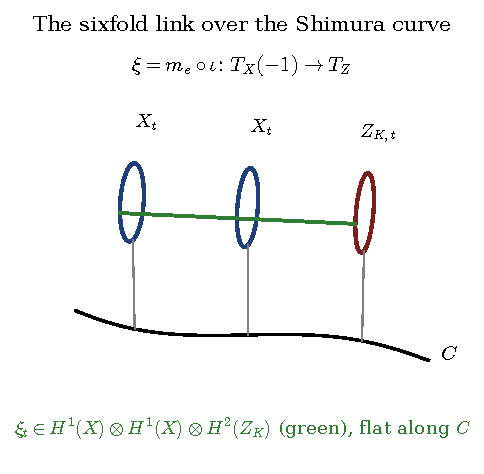
\includegraphics[width=0.78\textwidth]{figures/fig_link}
\caption{The sixfold link. Two copies of the Mumford fourfold $X_{t}$ and the sixfold $Z_{K,t}$ sit over the same point $t$ of the Shimura curve $C$; the class $\xi_{t}$ in the mixed K\"unneth component identifies the two copies of $T$ and is flat along $C$.}
\label{fig:link}
\end{figure*}

\begin{theorem}[The sixfold link]\label{thm:link}
Let $\xi$ be a nonzero element of $\Hom_{\Hdg}(T_{X}(-1),T_{Z})\subseteq H^{4}(X\times X\times Z_{K})$.
\begin{enumerate}[label=\textup{(\roman*)},leftmargin=2.4em,itemsep=2pt]
\item $\Hom_{\Hdg}(T_{X}(-1),T_{Z})=F\cdot\iota$ for the identification $\iota$ of Lemma~\ref{lem:tz}, so $\xi=m_{e}\circ\iota$ for a unique $e\in F^{\times}$. The $G\times K^{1}$-invariant classes of degree four on $X\times X\times Z_{K}$ have dimension $26$, and $\xi$ and $\psi\otimes\NS(Z_{K})$ are the only ones in the K\"unneth component $H^{1}(X)\otimes H^{1}(X)\otimes H^{2}(Z_{K})$.
\item If $\xi$ is algebraic, then $\xi^{\dagger}\xi$, the composite with the adjoint for the Lefschetz pairing on $X\times X$ and the intersection pairing on $Z_{K}$, is an algebraic endomorphism of $T_{X}(-1)$ equal to $m_{a(e)}$ with $a(e)=\kappa\,e^{2}c^{2}\in F$, $\kappa\in\QQ^{\times}$.
\item If $a(e)\notin\QQ$, the exceptional classes of $X\times X$ are algebraic at $t$, hence at every point of $C$, and so is every Hodge class on every power of $X$.
\item $a(e)\notin\QQ$ for every $e\in F^{\times}$ if and only if $K$ contains no imaginary quadratic field. If $K=F\cdot k$ with $k=\QQ(\sqrt{-d})$ and $c=f\sqrt{-d}$, then $a(e)\in\QQ$ exactly for $e\in\QQ f^{-1}$.
\item Conversely, if the exceptional classes are algebraic and some algebraic cycle on $X^{r}\times Z_{K}$ acts nonzero on $T_{Z}$, then every $\xi$ is algebraic.
\end{enumerate}
\end{theorem}

\begin{proof}
(i) Both sides are the irreducible $G$-representation $T$ with $\End_{\Hdg}=F$ \cite[Prop.~21.2]{BMB26}, so $\Hom_{\Hdg}=F\iota$. The count is the dimension of the kernel of the six raising and lowering operators of $\mathfrak{sl}_{2}^{3}$ on the torus-weight-zero part of $\bigwedge^{4}(V\oplus V\oplus D)$, computed by K\"unneth type: $(1,1,2)$ gives $3+3$, the line $F\iota$ and $\psi\otimes\NS(Z_{K})$; $(2,2,0)$ gives $4=\QQ\oplus F$, the Hodge classes of $X\times X$ in $H^{2}\otimes H^{2}$; $(0,0,4)$ gives $6=S^{2}\NS(Z_{K})$; $(2,0,2)$ and $(0,2,2)$ give $3$ each; and $(4,0,0)$, $(0,4,0)$, $(3,1,0)$, $(1,3,0)$ one each, products of divisor classes. The sum is $26$. The Hodge group of the product lies in $G\cdot K^{1}$, so $26$ bounds the Hodge classes from above; equality is not needed.

(ii) The adjoint of a correspondence for the Lefschetz pairing on $H^{2}(X\times X)$ and the polarised intersection pairing on $Z_{K}$ is the transposed cycle composed with cup products with powers of the polarisations and the inverse Lefschetz isomorphism, which is algebraic on an abelian variety \cite[\S2]{Kle68}; so $\xi^{\dagger}\xi$ is algebraic. By Lemma~\ref{lem:tz}, $T_{X}(-1)$ carries $-4q_{1}$ and $T_{Z}$ carries a rational multiple of $q_{c^{2}}$, and for $\xi=m_{e}$, $q_{c^{2}}(m_{e}x,m_{e}y)=\Tr(c^{2}e^{2}\trd(xy))=q_{1}(c^{2}e^{2}x,y)$, so $\xi^{\dagger}\xi=\kappa\,m_{e^{2}c^{2}}$.

(iii) An irrational $a\in F$ generates the cubic field, so every $m_{b}$, $b\in F$, is a polynomial in $\xi^{\dagger}\xi$, algebraic on $T_{X}(-1)$. Compose with the product map $\mu\colon H^{2}(X\times X)\supseteq T_{X}(-1)\to H^{2}(X)$ and its adjoint, both built from $\psi$, the diagonal and $\theta$ and hence algebraic \cite[Lem.~21.3]{BMB26}: the composite $\mu\circ(m_{b}\otimes1)\circ\mu^{\dagger}$ acts on the primitive part $U$ of $H^{2}(X)$ by the element $\nu(\Tr b-b)/2$ of $F$, irrational when $b$ is. With the identity and the projector onto $\QQ\theta$ this generates $\QQ\times F=\End_{\Hdg}H^{2}(X)$, so by \cite[Prop.~21.2]{BMB26} the exceptional classes are algebraic. The class $\xi$ is flat along $C$ and so are the exceptional classes, so by Lemma~\ref{lem:dichotomy} algebraicity at one point of the curve $C$ gives it on a countable set or everywhere; and \cite[Cor.~20.30]{BMB26} shows that algebraicity at one point of $C$ gives it at every point, and then every Hodge class on every power of $X$ is algebraic \cite[Thm.~21.7]{BMB26}.

(iv) $a(e)=\kappa e^{2}f^{2}\delta$ is rational iff $e^{2}f^{2}\delta\in\QQ$. If $-\delta\notin\QQ^{\times}(F^{\times})^{2}$ then $\delta\notin\QQ^{\times}(F^{\times})^{2}$ and $e^{2}f^{2}\delta\in\QQ$ is impossible. If $-\delta=-dg^{2}$ with $d\in\QQ^{\times}$, $g\in F^{\times}$, then with $c=f\sqrt{-d}$ one gets $a(e)=\kappa e^{2}f^{2}d$, rational iff $(ef)^{2}\in\QQ$ iff $ef\in\QQ$, a cubic field having no irrational element with rational square. And $-\delta\in\QQ^{\times}(F^{\times})^{2}$ exactly when $K\supseteq\QQ(\sqrt{-d})$ for some $d$.

(v) By \cite[Thm.~21.7]{BMB26} the Hodge conjecture holds for all powers of $X$ once the exceptional classes are algebraic. A cycle on $X^{r}\times Z_{K}$ acting nonzero on the irreducible $T_{Z}$ carries it isomorphically onto a summand of $H^{2k}(X^{r})(k-1)$; projecting onto that summand and composing with an isomorphism to $T_{X}(-1)\subseteq H^{2}(X\times X)$, a Hodge class on $X^{r+2}$ and algebraic, gives an algebraic nonzero element of $\Hom_{\Hdg}(T_{Z},T_{X}(-1))=F$; composing with the algebraic $m_{a}$ gives every element of that line, and transposing gives every $\xi$.
\end{proof}

\begin{proposition}[Hyper-K\"ahler carriers give $\pm1$]\label{prop:hk}
Let $Y_{1},\dots,Y_{m}$ be projective hyper-K\"ahler varieties of K3$^{[n_{j}]}$ type whose transcendental spaces are Hodge isometric to $(T,r_{j}q_{\lambda_{j}})$, $r_{j}\in\QQ^{\times}$, $\lambda_{j}\in F$ totally positive. Every composite of rational Hodge isometries between them that returns to $Y_{j}$ acts on $T$ by $\pm1$, and every composite of Hodge similarities by an element of $\QQ$.
\end{proposition}

\begin{proof}
A Hodge isometry $(T,r_{j}q_{\lambda_{j}})\to(T,r_{k}q_{\lambda_{k}})$ is a Hodge endomorphism of $T$, hence $m_{a}$ for some $a\in F$, and it is an isometry iff $r_{j}\lambda_{j}=r_{k}\lambda_{k}a^{2}$. A composite returning to $j$ is $m_{a}$ with $a^{2}=1$, and a composite of similarities is $m_{a}$ with $a^{2}\in\QQ$, which in a cubic field forces $a\in\QQ$. The isometries are algebraic by \cite{Bus19,Mar24}, which is why the statement matters: they realise $m_{b}$ between $S_{\lambda}$ and $S_{\lambda b^{-2}}$ and between their moduli spaces of sheaves, but every return is trivial.
\end{proof}

\subsection{Where the link stops}\label{ssec:f2stop2}

Theorem~\ref{thm:link} replaces the Kuga--Satake variety of \cite[Thm.~21.4]{BMB26}, of dimension $2^{7}$, by an abelian sixfold over the same curve, and it replaces the irrationality that had to be extracted from anticommuting Clifford blocks by the arithmetic of $K$: for every $K$ that is not a compositum $F\cdot k$ every link closes the target. Its logical status is the same as the Kuga--Satake link: by (v) it is equivalent to the target together with one algebraic link, not a reduction to something smaller.

The missing step is the algebraicity of one class $\xi\in H^{4}(X\times X\times Z_{K})$. It is exceptional: its component in $V\otimes V$ is the nine-dimensional $T$, not a multiple of $\psi$, so it is not invariant under $\Sp(V)$ and not in the Lefschetz algebra of $X\times X\times Z_{K}$ (Lemma~\ref{lem:sp-invariance}); the theorems that prove the conjecture when the Hodge ring is generated by divisors do not apply, and no Weil class of $Z_{K}$ or of $X\times X$ is involved. At the points of complex multiplication of $C$ the class $\xi_{c}$ is a Hodge class on a CM abelian variety in a mixed K\"unneth component between $X_{c}\times X_{c}$ and $Z_{K,c}$ with $\Hom(X_{c},Z_{K,c})=0$, so it is not a pull-back from one factor nor a product of lower-degree Hodge classes, and the generation theorems for CM abelian varieties do not reach it either. Unlike the Kuga--Satake class, the link is therefore not known even at the countably many special points. This is the price of staying inside abelian varieties, and it is the exact statement that \Fii{} needs at its smallest instance.
